% Template for an EarthArXiv preprint of the manuscript.
% Includes the standard disclaimers and formatting that is required.
%
% This is the document structure. The actual content is written in:
% * abstract.tex: The abstract.
% * abstract-plain.tex: A plain language version of the abstract.
% * content.tex: The actual manuscript text (minus the abstract).
%
%%%%%%%%%%%%%%%%%%%%%%%%%%%%%%%%%%%%%%%%%%%%%%%%%%%%%%%%%%%%%%%%%%%%%%%%%%%%%%%
% Set a class and general configuration
\documentclass[onecolumn,10pt]{article}

%%%%%%%%%%%%%%%%%%%%%%%%%%%%%%%%%%%%%%%%%%%%%%%%%%%%%%%%%%%%%%%%%%%%%%%%%%%%%%%
% Set variables with the title, authors, etc.
\newcommand{\Title}{The long version of the paper title}
\newcommand{\TitleShort}{A short title}

\newcommand{\Year}{2023}
\newcommand{\SubmittedOn}{2023/02/28}
\newcommand{\PublishedOn}{2023/02/28}

\newcommand{\AuthorShort}{Souza-Junior \textit{et al.}}
\newcommand{\Authors}{%
  Gelson F. Souza-Junior\textsuperscript{1},
  Leonardo Uieda\textsuperscript{1},
  Ricardo I. F. Trindade\textsuperscript{1},
  Yago M. Castro\textsuperscript{1}
}
\newcommand{\Email}{gelson.ferreira@usp.br}
\newcommand{\Corresponding}{%
  Corresponding author: Gelson F. Souza-Junior <\href{mailto:\Email}{\Email}>
}
\newcommand{\Affiliations}{%
  \textsuperscript{1} Universidade de São Paulo, Brazil;
}

\newcommand{\Journal}{Geochemistry, Geophysics, Geosystems}
\newcommand{\JournalDOI}{YYYYY/YYYYYYY}
\newcommand{\PreprintDOI}{XXXXX/XXXXXXX}
\newcommand{\ArchiveDOI}{DOI_FOR_THE_REPO_ARCHIVE}
\newcommand{\GitHubRepository}{compgeolab/paper-template}

\newcommand{\Keywords}{%
  keyword1; keyword2; keyword3;
}

%%%%%%%%%%%%%%%%%%%%%%%%%%%%%%%%%%%%%%%%%%%%%%%%%%%%%%%%%%%%%%%%%%%%%%%%%%%%%%%
% Import the required packages
\usepackage[utf8]{inputenc}
\usepackage[TU]{fontenc}
\usepackage[english]{babel}
\usepackage{amsmath}
\usepackage{amssymb}
\usepackage{graphicx}
\usepackage{hyperref}
\usepackage{fancyhdr}
\usepackage{orcidlink}
\usepackage{geometry}
\usepackage{booktabs}
\usepackage{microtype}
\usepackage{siunitx}
% To customize the title page
\usepackage{titling}
% For adding multiple authors
\usepackage{authblk}
% improved urls with proper hyphenation
\usepackage{xurl}
% Tweak the look of captions
\usepackage{caption}
% To control the style of section titles
\usepackage{titlesec}
% Import natbib and doi packages
\usepackage[round,authoryear,sort]{natbib}
% show dois as links on references
\usepackage{doi}
% Remove extra space between references
\usepackage{natbibspacing}
% Use a different font
\usepackage[scaled=1.1]{notomath}
% Icons and fonts (requires using xelatex or luatex)
\usepackage{fontawesome5}
\usepackage{academicons}
% Control the font size
\usepackage{anyfontsize}
\usepackage{setspace}
% To get the number of pages in the document
\usepackage{lastpage}
\usepackage{lipsum}
\usepackage{ragged2e}
\usepackage{mdframed}
% To define custom environments
\usepackage{environ}
% To control hyphenation for individual blocks of text
\usepackage{hyphenat}


%%%%%%%%%%%%%%%%%%%%%%%%%%%%%%%%%%%%%%%%%%%%%%%%%%%%%%%%%%%%%%%%%%%%%%%%%%%%%%%
% Configuration of the document

\geometry{%
  left=25mm,
  right=25mm,
  top=18mm,
  bottom=15mm,
  headsep=0mm,
  headheight=0mm,
  footskip=7mm,
  includehead=true,
  includefoot=true
}

% Control line and table row spacing
\onehalfspacing
\renewcommand{\arraystretch}{1.5}

% Set the spacing between bibliography entries (requires natbib)
\setlength{\bibsep}{0pt}

% Custom colors
\definecolor{darkgray}{gray}{0.4}
\definecolor{mediumgray}{gray}{0.5}
\definecolor{lightgray}{gray}{0.9}
\definecolor{mediumblue}{HTML}{2060c2}
\definecolor{lightblue}{HTML}{f7faff}

% Configure captions
\captionsetup[table]{position=below,skip=0pt}
\captionsetup{labelfont=bf,font={small,color=darkgray},skip=10pt}

% Make urls use the same font as every other text
\urlstyle{same}

% Configure hyperref and add PDF metadata
\hypersetup{
    colorlinks,
    allcolors=mediumblue,
    pdftitle={\Title},
    pdfauthor={\AuthorShort},
    breaklinks=true,
}

% Configure header and footer
% Inspired by LaPreprint: https://github.com/roaldarbol/LaPreprint
\newcommand{\Separator}{\hspace{3pt}|\hspace{3pt}}
\newcommand{\FooterFont}{\footnotesize\color{mediumgray}}
\pagestyle{fancy}
\fancyhf{}
\lfoot{%
  \FooterFont{}
  \AuthorShort{} (\Year)
  \Separator{}
  \TitleShort
}
\rfoot{%
  \FooterFont{}
  EarthArXiv
  \Separator{}
  \thepage\space of\space \pageref*{LastPage}
}
\renewcommand{\headrulewidth}{0pt}
\renewcommand{\footrulewidth}{1pt}
\preto{\footrule}{\color{lightgray}}
\fancypagestyle{plain}{%
  \fancyhf{}
  \lfoot{%
    \FooterFont{}
    \faCreativeCommons\faCreativeCommonsBy
    \Separator{}
    \textcopyright{} \Year{} The Authors
  }
  \rfoot{%
    \FooterFont{}
    doi:\href{https://doi.org/\PreprintDOI}{\PreprintDOI}
    \Separator{}
    EarthArXiv
    \Separator{}
    \thepage\space of\space \pageref*{LastPage}
  }
}

% Define fancy text boxes
\NewEnviron{summarybox}{%
  \mdfdefinestyle{summarybox_}{%
    leftline=true,
    rightline=false,
    topline=false,
    bottomline=false,
    linewidth=2pt,
    linecolor=mediumblue,
    backgroundcolor=lightblue,
    innertopmargin=12pt,
    innerbottommargin=12pt,
    innerleftmargin=12pt,
    innerrightmargin=12pt,
    skipbelow=5pt,
    skipabove=5pt,
  }
  \newmdenv[style=summarybox_]{summarybox_}
  \begin{summarybox_}
    \footnotesize
    \BODY
  \end{summarybox_}
}

%%%%%%%%%%%%%%%%%%%%%%%%%%%%%%%%%%%%%%%%%%%%%%%%%%%%%%%%%%%%%%%%%%%%%%%%%%%%%%%
\begin{document}

\thispagestyle{plain}
\begin{FlushLeft}
  \begin{spacing}{2}
    {\LARGE\bfseries \Title}
  \end{spacing}
  {\color{lightgray}\hrule height 1.5pt}
  \vspace{0.3cm}
  \Authors
  \\[0.2cm]
  {\footnotesize \Affiliations}
  \newline
  {\footnotesize \Corresponding}
  \\[0.2cm]
  {\footnotesize
    Received in original form on \SubmittedOn.
    %Published in final form on \PublishedOn.
  }
\end{FlushLeft}

\begin{summarybox}
  \noindent
  \textbf{Disclaimer:}
  %This is a non-peer reviewed preprint of an article submitted for publication
  %in \textit{\Journal{}}. It is available from EarthArXiv at
  %\url{https://doi.org/\PreprintDOI}.
  %%%%%%%%%%%%%%%%%%%%%%%%%%%%%%%%%%%%%%%%%%%%%%%%%%%%%%%%%%%%%%%%%%%%%%%%%%%%%
  % Comment the above and uncomment below after publication in a journal
  %%%%%%%%%%%%%%%%%%%%%%%%%%%%%%%%%%%%%%%%%%%%%%%%%%%%%%%%%%%%%%%%%%%%%%%%%%%%%
  This is a peer-reviewed author-produced postprint of the article
  ``\AuthorShort{} (\Year). \Title. \textit{\Journal}.
  doi:\href{https://doi.org/\JournalDOI}{\JournalDOI}''.
  The postprint is available from EarthArXiv at
  \url{https://doi.org/\PreprintDOI}.
  %%%%%%%%%%%%%%%%%%%%%%%%%%%%%%%%%%%%%%%%%%%%%%%%%%%%%%%%%%%%%%%%%%%%%%%%%%%%%
  \\[0.25cm]
  \noindent
  \textbf{Open research:}
  The source code used to generate all of the results presented in this
  research can be freely accessed and reused under the terms of an open license.
  You can find it at \url{https://doi.org/\ArchiveDOI} and
  \url{https://github.com/\GitHubRepository}.
  \\[0.25cm]
  \noindent
  \textbf{Keywords:} \Keywords{}
  \\[0.25cm]
  \noindent
  \textbf{\textcopyright{} \Year{} The Authors.}
  Available under the \href{https://creativecommons.org/licenses/by/4.0/}{Creative Commons Attribution 4.0 International License}
  \faCreativeCommons\faCreativeCommonsBy{}.
\end{summarybox}

\section*{\normalsize Plain language summary}
\begingroup
  \setstretch{1.1} \small \lipsum[3]
 \par
\endgroup

\section*{\normalsize Abstract}
\begingroup
  \setstretch{1.1} \small Magnetic microscopy mapping for paleomagnetic studies has attracted considerable attention in recent years due to its high accuracy and robustness. However, due to the nature of the magnetic field, it is difficult to accurately estimate the magnetic source's position and dipole moment. This study proposes a new methodology to mitigate the magnetic sources' interference and enhance the precision of the inversion analyses proposed. The proposed methodology is based on refining the isolation of the primary signal and integrating the "interfering sources" algorithm, which addresses one of the previous code's limitations. Moreover, the proposed methodology was applied to synthetic data to assess the algorithm's reliability and precision, reinforcing the advancement of paleomatrix data analysis and setting a definitive path for future enhancements. \par
\endgroup

\section{Introduction}

Since the pioneering contributions of \citet{Egli2000}, implementing high-resolution  magnetic microscopy (MM) methodologies to paleomagnetic analysis has become increasingly feasible in paleomagnetic research. This has offered an alternative to conventional paleomagnetic approaches that typically analyze entire, centimeter-scale rock samples. Magnetic microscopy allows better characterization of magnetization heterogeneities, which are usually undetectable by classical paleomagnetic analysis, as the magnetometers measure the contribution of all magnetic carriers in the rock at once. Although MM techniques provide a magnetically resolved perspective to each source, processing the measured field can be very challenging. Potential field data are naturally associated with ambiguities, which generate non-unique solutions during inversion procedures that aim to recover the magnetic moment of these sources \citep{Blakely1996}. A standard routine applied to circumvent the non-uniqueness is integrating prior knowledge about the sources causing the anomaly. X-ray computed tomography (microCT) -- which determines the position of magnetic grains within a sample \citep{Fabian2019} -- is an example of such prior information \citep[\textit{e.g.}][]{DeGroot2018, DeGroot2021, Koster2023}, which can then be incorporated into the inversion of the magnetic moment by using spherical harmonic expansions \citep[\textit{e.g.}][]{CortesOrtuno2021, CortesOrtuno2022}.

Another way to incorporate additional information to the inverse problem without performing new measurements was proposed by \citet{Souza-Junior2024}. Their methodology borrows processing and interpretation techniques of aeromagnetic surveys, such as the Euler deconvolution and field transformations, since the data are similar to magnetic microscopy \citep{Weiss2007}. The methodology was designed for the semi-automatic estimation of position and dipole moments for individual grains and consists of three main steps. First, it combines classic potential field data processing (like total gradient amplitude) with image processing techniques (namely, histogram stretching and blob detection) to identify and isolate the magnetic fields of individual sources into data windows. Next, the 3D position of the source is estimated through the Euler deconvolution method \citep{Reid1990} based on the magnetic microscopy field measurements within each data window. Finally, the 3-component dipole moment vector is obtained using a least-square estimator assuming that a dipolar source causes the magnetic anomaly \citep{Oliveira2015Estimation}. The methodology was originally designed for computational efficiency and stability. However, it infringes on the mathematical premise of inversion theory, which states that the sampled area must be encapsulated by the inversion domain \citep{Baratchart2013, Lima2013}. Thus, more often than not, it fails to account for the mutual interference between sources and shifts in the measured field. This study introduces significant modifications to the method of \citet{Souza-Junior2024} that aim to account for the mutual interference of the sources, as well as any shift in the field. Through refining the window-based approach, the proposed methodology is able to more accurately recover the dipole moments and positions of a larger number of sources than the previous method. We tested the improved method in synthetic and real magnetic microscopy data, showing its applicability to micropaleomagnetic analysis.


%%%%%%%%%%%%%%%%%%%%%%%%%%%%%%%%%%%%%%%%%%%%%%%%%%%%%%%%%%%%%%%%%%%%%%%%%%%%%%%
\section{Methods}

We propose modifications to the methodology of \citet{Souza-Junior2024} to improve its accuracy in scenarios where signals from neighboring particles overlap, causing distortions in the signal of the weaker particles and biasing the source detection and dipole moment inversion results (as shown in Figure~\ref{method-redetection}a). The new method uses the following workflow:

\begin{enumerate}
    \item \textbf{Source detection:} We use the same procedure described in \citet{Souza-Junior2024}, namely calculating the total-gradient amplitude of the magnetic data, histogram stretching, and a blob detection algorithm. This produces a set of data windows that contain the observed signals of individual particles.
    \label{alg:workflow-detection}
    \item \textbf{Sort the data windows} by order of decreasing signal strength and perform the following steps on each window following this order:
    \label{alg:workflow-loop}
    \begin{enumerate}
        \item \textbf{Isolate the data:} Select the portion of the magnetic data that falls inside the current data window. The following steps are performed on this selected dataset.
        \item {Euler:}
        \item \textbf{Linear magnetic moment inversion:} Perform a linear inversion to estimate the dipole moment of the source using the Euler deconvolution solution as prior information to fix the source position.
        \item \textbf{Non-linear inversion:} Unlike \citet{Souza-Junior2024}, we then refine the position and dipole moment estimates by a non-linear inversion using the Nelder-Mead method \citep{Nelder-Mead1965,Gao2010}. The Euler deconvolution and linear inversion results are used as initial estimates for the optimization.
        \item \textbf{Signal removal:} Forward model the magnetic field of the estimated dipole from the previous step and remove the signal from the full magnetic data.
    \end{enumerate}
    \item Now, the original magnetic data has been stripped of the signal of all detected sources. Repeat steps~\ref{alg:workflow-detection} and \ref{alg:workflow-loop} on the stripped dataset to detect new sources and determine their positions and dipole moments.
\end{enumerate}

\noindent
Below, we describe these steps in more detail.

\subsection{Position estimation}
    Euler deconvolution (ED) \citep{Reid1990} is a procedure widely applied in aeromagnetic surveys \citep{Barbosa2011, Melo2013} to obtain a 3D position estimation of the magnetic source. The only assumption is the source's shape given by the structural index ($\eta$).
    In the case of a dipole $\eta = 3$. Euler deconvolution is based on Euler's homogeneity equation

        \begin{equation}
        \label{eq_euler_homogeneity}
        (x - x_c)\partial_x f
        + (y - y_c)\partial_y f
        + (z - z_c)\partial_z f
        = (b - f)\eta
        \ ,
        \end{equation}

    \noindent
    in which $(x, y, z)$ are the observation point coordinates in a Cartesian system, $(x_c, y_c, z_c)$ are the coordinates of the source, $b$ is a constant shift in the data called the \textit{base level}, $\eta$ is the structural index, and $f$ is the magnetic field.
    The equation above can be rearranged to isolate the unknown source position  and the base level

    \begin{equation}
    x_c \partial_x f + y_c \partial_y f + z_c \partial_z f + \eta b
    =
    x \partial_x f + y \partial_y f + z \partial_z f + \eta f
    \ .
    \end{equation}

    Given $N$ observation of the magnetic field and its $x$-, $y$-, and $z$-derivatives, we can form a $N \times 4$ system of equations

    \begin{equation}
    {\overbrace{
    \begin{bmatrix}
      {\partial_x f}_1 & {\partial_y f}_1 & {\partial_z f}_1 & \eta \\
      {\partial_x f}_2 & {\partial_y f}_2 & {\partial_z f}_2 & \eta \\
      \vdots & \vdots & \vdots & \vdots \\
      {\partial_x f}_N & {\partial_y f}_N & {\partial_z f}_N & \eta
    \end{bmatrix}
    }^{\mathbf{G}}}_{N \times 4}
    {\overbrace{
    \begin{bmatrix}
      x_c \\ y_c \\ z_c \\ b
    \end{bmatrix}
    }^{\mathbf{p}}}_{4 \times 1}
    =
    {\overbrace{
    \begin{bmatrix}
      x_1 {\partial_x f}_1 + y_1 {\partial_y f}_1 + z_1 {\partial_z f}_1 + \eta f_1 \\
      x_2 {\partial_x f}_2 + y_2 {\partial_y f}_2 + z_2 {\partial_z f}_2 + \eta f_2 \\
      \vdots \\
      x_N {\partial_x f}_N + y_N {\partial_y f}_N + z_N {\partial_z f}_N + \eta f_N \\
    \end{bmatrix}
    }^{\mathbf{h}}}_{N \times 1}
    \ ,
    \end{equation}

    \noindent
    in which $\mathbf{G}$ is the Jacobian matrix, $\mathbf{p}$ is the parameter vector, and $\mathbf{h}$ is the pseudo-data vector.

    The least-squares solution of this linear system is defined by the vector $\mathbf{p}$ that minimizes the misfit function, $\phi(\mathbf{p})$, given by the sum of the squared differences between the observed pseudo-data vector $\mathbf{h}^o$ and the predicted pseudo-data vector $\mathbf{h}$

    \begin{equation}
    \label{function_phi}
    \phi(\mathbf{p})
    = \| \mathbf{h}^o - \mathbf{h} \|_2^2\
    = \| \mathbf{h}^o - \mathbf{G}\mathbf{p} \|_2^2\
    \ .
    \end{equation}

    \noindent
    The solution that minimizes the misfit function is

    \begin{equation}
    \label{euler_solution}
    \mathbf{p} = \left(\mathbf{G}^T \mathbf{G}\right)^{-1} \mathbf{G}^T \mathbf{h}^o\ .
    \end{equation}

    \noindent
    The parameter vector $\mathbf{p}$ contains the coordinates of the dipolar source $(x_c, y_c, z_c)$, as well as the base level $b$, which is the background field within the data window.

\subsection{Linear magnetic moment inversion}

     Following \citet{Oliveira2015Estimation} and \citet{Souza-Junior2024}, the vertical component of the magnetic field $f_z$ has a linear relationship with the dipole moment components $(m_x, m_y, m_z)$ given by the following matrix equation

     \begin{equation}
    \label{eq_dipole_bz}
    {\overbrace{\begin{bmatrix}
    \dfrac{\mu_0}{4\pi} \dfrac{\partial^2}{\partial z \partial x} \dfrac{1}{r_1}
    & \dfrac{\mu_0}{4\pi} \dfrac{\partial^2}{\partial z \partial y} \dfrac{1}{r_1}
    & \dfrac{\mu_0}{4\pi} \dfrac{\partial^2}{\partial z^2} \dfrac{1}{r_1}
    \\
    \vdots & \vdots & \vdots
    \\
    \dfrac{\mu_0}{4\pi} \dfrac{\partial^2}{\partial z \partial x} \dfrac{1}{r_i}
    & \dfrac{\mu_0}{4\pi} \dfrac{\partial^2}{\partial z \partial y} \dfrac{1}{r_i}
    & \dfrac{\mu_0}{4\pi} \dfrac{\partial^2}{\partial z^2} \dfrac{1}{r_i}
    \\
    \vdots & \vdots & \vdots
    \\
    \dfrac{\mu_0}{4\pi} \dfrac{\partial^2}{\partial z \partial x} \dfrac{1}{r_N}
    & \dfrac{\mu_0}{4\pi} \dfrac{\partial^2}{\partial z \partial y} \dfrac{1}{r_N}
    & \dfrac{\mu_0}{4\pi} \dfrac{\partial^2}{\partial z^2} \dfrac{1}{r_N}
    \end{bmatrix}}^{\mathbf{A}}}_{N \times 3}
    {\overbrace{{\begin{bmatrix}
    m_x \\ m_y \\ m_z
    \end{bmatrix}}}^{\mathbf{m}}}_{3 \times 1}
    =
    ~{\overbrace{\begin{bmatrix}
    {f_z}_1
    \\
    \vdots
    \\
    {f_z}_i
    \\
    \vdots
    \\
    {f_z}_N
    \end{bmatrix}}^{\mathbf{d}}}_{N \times 1}
    \ ,
    \end{equation}

    \noindent
    in which $r_i = \sqrt{(x_i - x_c)^2 + (y_i - y_c)^2 + (z_i - z_c)^2}$ is the distance between the observation point $(x_i, y_i, z_i)$ and the dipolar source $(x_c, y_c, z_c)$, $\mu_0$ is the vacuum magnetic permeability, matrix $\mathbf{A}$ is the Jacobian matrix, vector $\mathbf{m}$ is the parameter vector containing the dipole moment components, and $\mathbf{d}$ is the predicted data vector. The second-order derivative terms in Equation~\ref{eq_dipole_bz} are

    \begin{equation}
    \begin{aligned}
    \dfrac{\partial^2}{\partial z \partial x} \dfrac{1}{r_i} &=
    \dfrac{3(z_i - z_c)(x_i - x_c)}{{r_i}^5}\ ,
    \\
    \dfrac{\partial^2}{\partial z \partial y} \dfrac{1}{r_i} &=
    \dfrac{3(z_i - z_c)(y_i - y_c)}{{r_i}^5}\ ,
    \\
    \dfrac{\partial^2}{\partial z^2} \dfrac{1}{r_i} &=
    \dfrac{3(z_i - z_c)^2}{{r_i}^5} - \dfrac{1}{{r_i}^3}\ .
    \end{aligned}
    \end{equation}

    The least-squares solution to the linear system in  Equation~\ref{eq_dipole_bz} is the parameter vector $\mathbf{m}$ that minimizes the misfit function $\psi(\mathbf{m})$, which is given by the sum of the squared differences between the observed  $\mathbf{d}^o$ and predicted $\mathbf{d}$ data vectors

    \begin{equation}
    \label{psi_function}
    \psi(\mathbf{m})
    = \min_{\mathbf{m}} \| (\mathbf{d}^o - b) - \mathbf{d} \|_2^2
    = \| (\mathbf{d}^o - b) - \mathbf{A}\mathbf{m} \|_2^2\
    \ .
    \end{equation}

    \noindent
    The background field $b$ estimated by Euler deconvolution is removed from the observed data to account for static shifts in the microscopy data which cannot be replicated by a dipolar field.

    The parameter vector $\mathbf{m}$, containing the Cartesian components of the magnetic moment, that minimizes the misfit function $\psi$ is

    \begin{equation}
    \label{dipole_moment_solution}
    \mathbf{m} = \left(\mathbf{A}^T \mathbf{A}\right)^{-1} \mathbf{A}^T (\mathbf{d}^o - b)\ .
    \end{equation}


\subsection{Non-linear inversion}

    The presence of signals from interfering sources in the current data window can cause biases in the Euler deconvolution position estimate \citep{Uieda2025}, which in turn are propagated to the estimated dipole moment by linear inversion.
    To help mitigate this interference, we employ a non-linear inversion to estimate the dipole moment and source position simultaneously.

     After obtaining the estimates of the 3D position $\mathbf{x} = [x_{c}\ y_{c}\ z_{c}]^T$ from Euler deconvolution and the dipole moment vector $\mathbf{m} = [m_{x}\ m_{y}\ m_{z}]^T$ from the linear inversion, we formulate a new non-linear misfit function $\xi(\mathbf{x}, \mathbf{m})$

    \begin{equation}
    \label{misfit_equation}
    \xi(\mathbf{x}, \mathbf{m}) =
    \| (\mathbf{d}^o - b) - \mathbf{d}(\mathbf{x}, \mathbf{m}) \|_2^2.
    \end{equation}

    \noindent
    in which $\mathbf{d}(\mathbf{x}, \mathbf{m})$ is the forward model from Equation~\ref{eq_dipole_bz}.

    The solutions $\mathbf{x}$  and $\mathbf{m}$ that minimize the misfit function above can be estimated through a non-linear optimization method.
    Here, we use the Nelder-Mead method \citep{Nelder-Mead1965,Gao2010} with initial estimates of $\mathbf{x}$ and $\mathbf{m}$ from Euler deconvolution and the linear dipole moment inversion, respectively.
     The Nelder-Mead method is a gradient-free optimization technique, which systematically searches the optimal solution of Equation~\ref{misfit_equation} by iteratively adjusting a simplex in the parameter space \citep{Nelder-Mead1965}. This is particularly useful for optimizing functions where gradients are difficult or impractical to compute.

     However, the substantial difference of up to seven orders of magnitude between the position and the magnetic moment poses a challenge. This dissimilarity directly affects the simplex operations and can prevent the algorithm from converging. We address this problem by normalizing the magnetic moment by the magnitude of the initial estimate

    \begin{align}
    \label{normalizing_m_parameters}
    m_0 &= \sqrt{{m_x}_0^2+{m_y}_0^2+{m_z}_0^2}\ ,
    & {m_x}^{j+1} &= \frac{{m_x}^{j}}{m_0},
    & {m_y}^{j+1} &= \frac{{m_y}^{j}}{m_0},
    & \text{and} &
    & {m_z}^{j+1} &= \frac{{m_z}^{j}}{m_0}
    \ .
    \end{align}

\noindent
Which was also applied for the position vector using the initial position estimates:

\begin{align}
\label{normalizing_h_parameters}
{x_c}^{j+1} &= \frac{{x_c}^{j}}{{x_c}_0},
& {y_c}^{j+1} &= \frac{{y_c}^{j}}{{y_c}_0},
& \text{and} &
&{z_c}^{j+1} &= \frac{{z_c}^{j}}{{z_c}_0}
\ .
\end{align}

\noindent
These normalization procedures ensure that each parameter falls within a unit range for a given number M of iterations of the simplex optimization, $j = 1,2,..., M$.


\subsection{Signal removal}
\label{sec:signal_removal}

    A logical route to account for mutual interference between magnetic sources would be solving the magnetic moment for the whole of the sources at the same time. However, this approach raises three main concerns:

    \begin{enumerate}
        \item \textbf{The size of the problem:} A linear problem $N \times 3L$ ($N$ being the number of observed data points and $L$ the number of sources) would be obtained in Equation~\ref{eq_dipole_bz}. This poses a problem because the magnetic microscopy data includes a large number of observation points and potentially encompassing hundreds to thousands of identified sources. Therefore, working with sliced windowed data requires less computational resources.

        \item \textbf{Background field correction:} In the proposed methodology, correction for the background field ($b$) eliminates the need for preprocessing the data for regional-residual separation to remove the effects of shifts in the magnetic data. This application is feasible because $b$ is also provided by the ED solution when using windowed data. Simultaneous inversion of all sources would require the removal of the regional field prior to inversion, which is difficult to do without biasing the estimated directions.

        \item \textbf{No visible advantage over windowed data}: Tests with synthetic data \citep[see supplementary Jupyter notebooks in][]{figshare} showed no significant advantage over windowed data. The latter performed significantly better in the benchmark and had lower processing times.

    \end{enumerate}

    Considering the above, a sequential subtraction of the magnetic carriers' influence is proposed to maintain the window-based approach. The magnetic signal associated with each identified source was computed using a dipole forward model (Equation~\ref{eq_dipole_bz}) and the estimated parameter vector. The forward-modeled signal of a stronger source was then selectively removed from the dataset, resulting in a dataset devoid of its influence at the current step.
    This is similar to the \texttt{subtract\_source} routine in the QDMlab software \citep{Volk2022}. This process allowed for the gradual isolation of weaker sources' contributions. The updated dataset was also used to recalculate the directional derivatives for the subsequent Euler deconvolution position estimation.

    This step-by-step procedure is subsequently employed for all detected particles in the sample, from the strongest magnetic signals to the weakest. This led to an improved position estimation compared to the original methodology of \citep{Souza-Junior2024}. This novel methodology, designed to mitigate the impact of stronger sources and with a better estimation of positions, significantly enhances the precision of subsequent inversion analyses. However, a trade-off between achieving better results and incurring longer computational runtime is unavoidable.

\subsection{Residual anomaly detection}

   The magnetic moment of a material is directly proportional to its volume. In a rock fabric, this can result in a wide range of particle diameter distributions, from small, stable recording grains (single domain, SD, e.g. around 60 nm for magnetite) to less reliable magnetic carriers (multi-domain, MD, greater than 1000 nm for the same mineral) \citep{Nagy2019}. This results in a significant contrast in the magnetic signal measured using the magnetic microscope. This effect is evident in the synthetic example shown in Figure~\ref{method-redetection}a, which features dipolar sources with a magnetic moment contrast spanning 5 orders of magnitude.

    In the original methodology \citep{Souza-Junior2024}, sources are initially identified for window selection using a total gradient anomaly (TGA) map, with contrast stretched to highlight sources of varying intensities (both strong and weak) as shown in Figure~\ref{method-redetection}b. However, due to the high signal contrast, this approach proved insufficient for identifying all relevant sources. To address this issue, the procedure outlined in Section~\ref{sec:signal_removal} was implemented to obtain a residual anomaly map. Reapplying the source detection algorithm to this new map enabled the identification of weaker sources (Figure~\ref{method-redetection}c), as the signal from stronger sources was effectively removed. This improvement resulted from the reduced disparity between the signals of weaker magnetic sources and the residual anomalies from each window inversion.

    \begin{figure}[tb!]
      \centering
      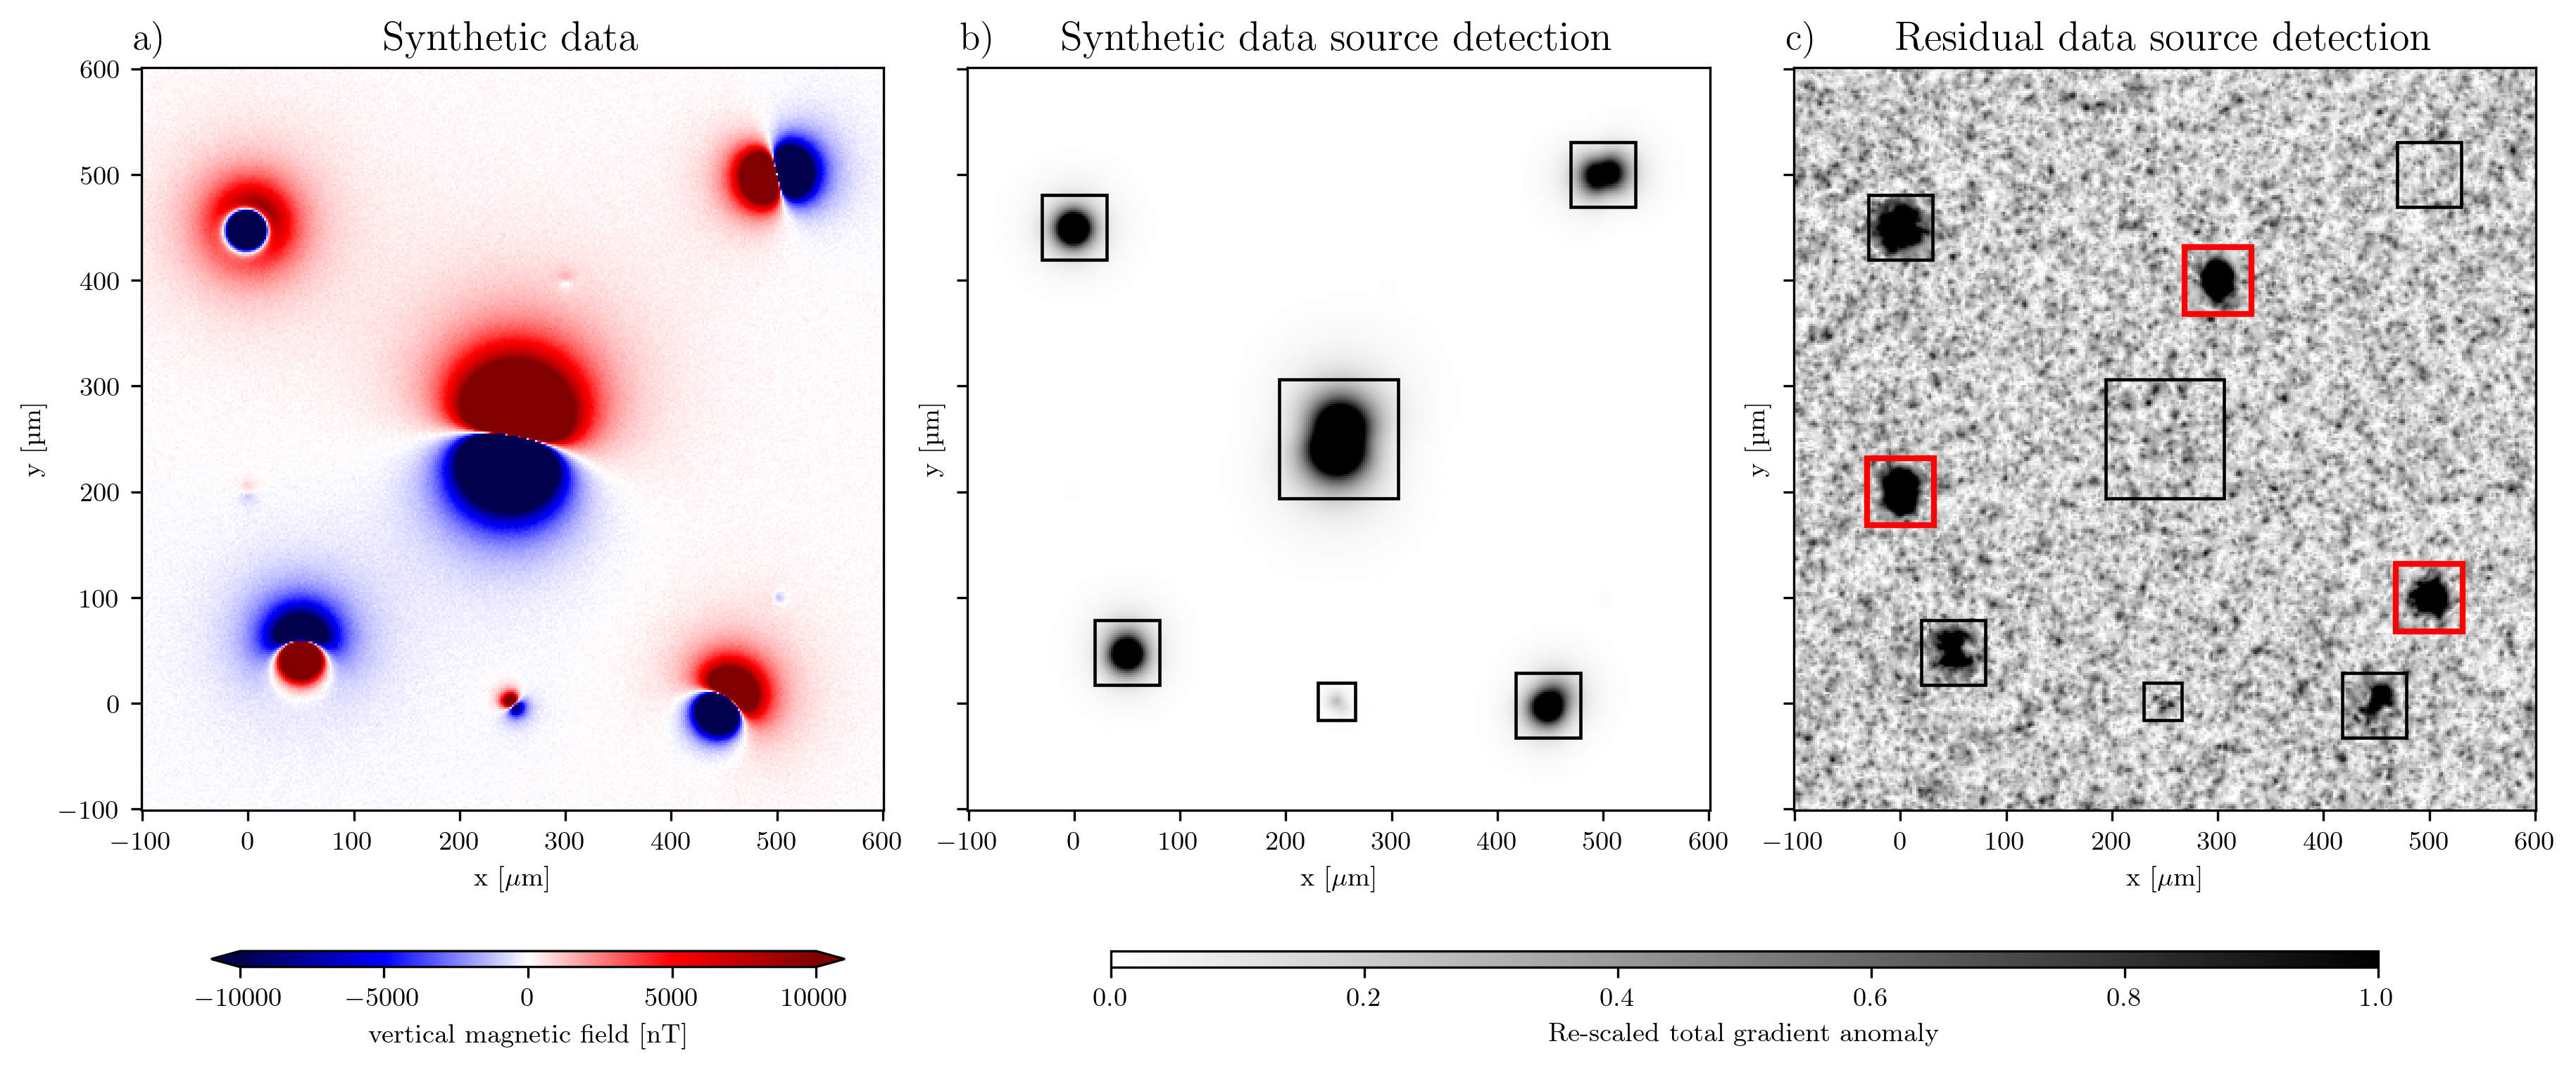
\includegraphics[width=1\linewidth]{figures/re-detection-methodology.png}
      \caption{Source detection workflow on the residual anomaly. a) Synthetic sample featuring a wide range of magnetic moment intensities. b) The Blob detection algorithm identify the sources by using the total gradient obtained with the vertical component of the magnetic field. c) Result of the blob detection algorithm when applied to the total gradient of the residual anomaly.}
      \label{method-redetection}
    \end{figure}

%%%%%%%%%%%%%%%%%%%%%%%%%%%%%%%%%%%%%%%%%%%%%%%%%%%%%%%%%%%%%%%%%%%%%%
\section{Numerical simulations}

In this section, we evaluate the effectiveness of the interfering sources method, in comparison with the method proposed by \citet{Souza-Junior2024}, by applying it to two synthetic datasets. The tests are structured as follows:

\begin{enumerate}
    \item \textbf{Evaluating overlapping signal detection:} This test simulates a single map containing both strong and weak sources to evaluate the the new methodology's effectiveness in discerning and accurately locating the weaker sources, despite the interferences causing by the stronger ones.

    \item \textbf{Assessing performance with variable particle density:} This test introduces a more complex scenario by simulating a specific magnetization direction for the magnetic sources. Additionally, three different particle density scenarios are modeled to test whether the method can reliably recover the magnetization direction across all cases.

\end{enumerate}

\subsection{Evaluating overlapping signal detection}
\label{sec:synthetic-overlapping}

The first model scenario consists of several dipole sources with varying moment magnitudes, inclinations, and declinations, organized into three distinct groups. The first group contains 150 dipoles with random orientations and moment magnitudes an order of magnitude larger than those in the second group. The second group comprises 50 dipoles with a stable orientation: an inclination of \(\ang{35}\) (\(\pm \ang{5}\)), a declination of \(\ang{340}\) (\(\pm \ang{5}\)), and dipole moment magnitudes centered at \(1.0 \times 10^{-16} Am^2\). Additionally, a third group includes 9 sporadic, deeper, and strongly magnetized sources with random orientations and significantly higher dipole moments of \(1.0 \times 10^{-11} Am^2\). Which totals 209 magnetic particles.

To evaluate the methodologies, we simulate these magnetic sources randomly distributed within a synthetic thin with a field of view section measuring \(\qty{2000}{\micro\meter} \times \qty{2000}{\micro\meter}\). The synthetic vertical magnetic field data (\(b_z\)) are generated on a regular grid with \(\qty{2}{\micro\meter}\) spacing and a sensor sample distance of \(\qty{5}{\micro\meter}\), without any external applied field. Thus, the magnetic anomaly is solely caused by their dipole moment. High-frequency (\(\qty{50}{\nano\tesla}\) following \citet{Glenn2017}), spatially correlated pseudo-random noise, modeled after the spectral characteristics of the blank 2070615-NID08 diamond map, was added to replicate typical experimental conditions of other diamonds, providing a realistic approximation of a QDM measurement. The modeled sources were positioned at depths ranging from 1 to \(\qty{20}{\micro\meter}\). To further emulate actual acquisition conditions, a positive baseline shift of \(\qty{400}{\nano\tesla}\) \citep[following][]{Hess2024} is applied to the magnetic field data. This setup tests the algorithm's robustness and accuracy when handling systematically shifted and noise-corrupted magnetic field measurements, as commonly observed in magnetic microscopy experiments.

The synthetic data inversion was resolved using both the standard method \citep{Souza-Junior2024} and the newly proposed interfering sources methodology. A summary comparison of the classic Euler method and the iterative approach showed significant results in analyzing the synthetic data. The iterative Euler deconvolution method notably enhanced source detectability, with newly identified windows highlighted (green squares, Figure \ref{euler2}a). Figure \ref{euler2}b displays the 112 sources initially detected from the 209 modeled. Meanwhile, Figure \ref{euler2}c indicates that the iterative Euler method retrieved 166 sources. Initially, it may appear that the improvements of the iterative method  over the standard one in terms of tridimensional source location precision were modest. Yet, most previously identified sources demonstrate reduced position misfit (barring sporadic deeper ones). The larger misfits in Figure \ref{euler2}c are linked to the newly identified grains (represented by the colored squares), as their smaller dipole moment results in greater error in the Euler estimation. This increase in accuracy is crucial, especially in scenarios where stronger magnetic sources can distort the magnetic field anomaly of weaker sources. Although this new methodology can markedly increase the accuracy in the estimated position for virtually all sources, the biggest errors are still related to clustered sources. Also, in both cases, the Euler deconvolution seems unaffected by the presence of a shift in the magnetic field.


\begin{figure}[tb!]
  \centering
  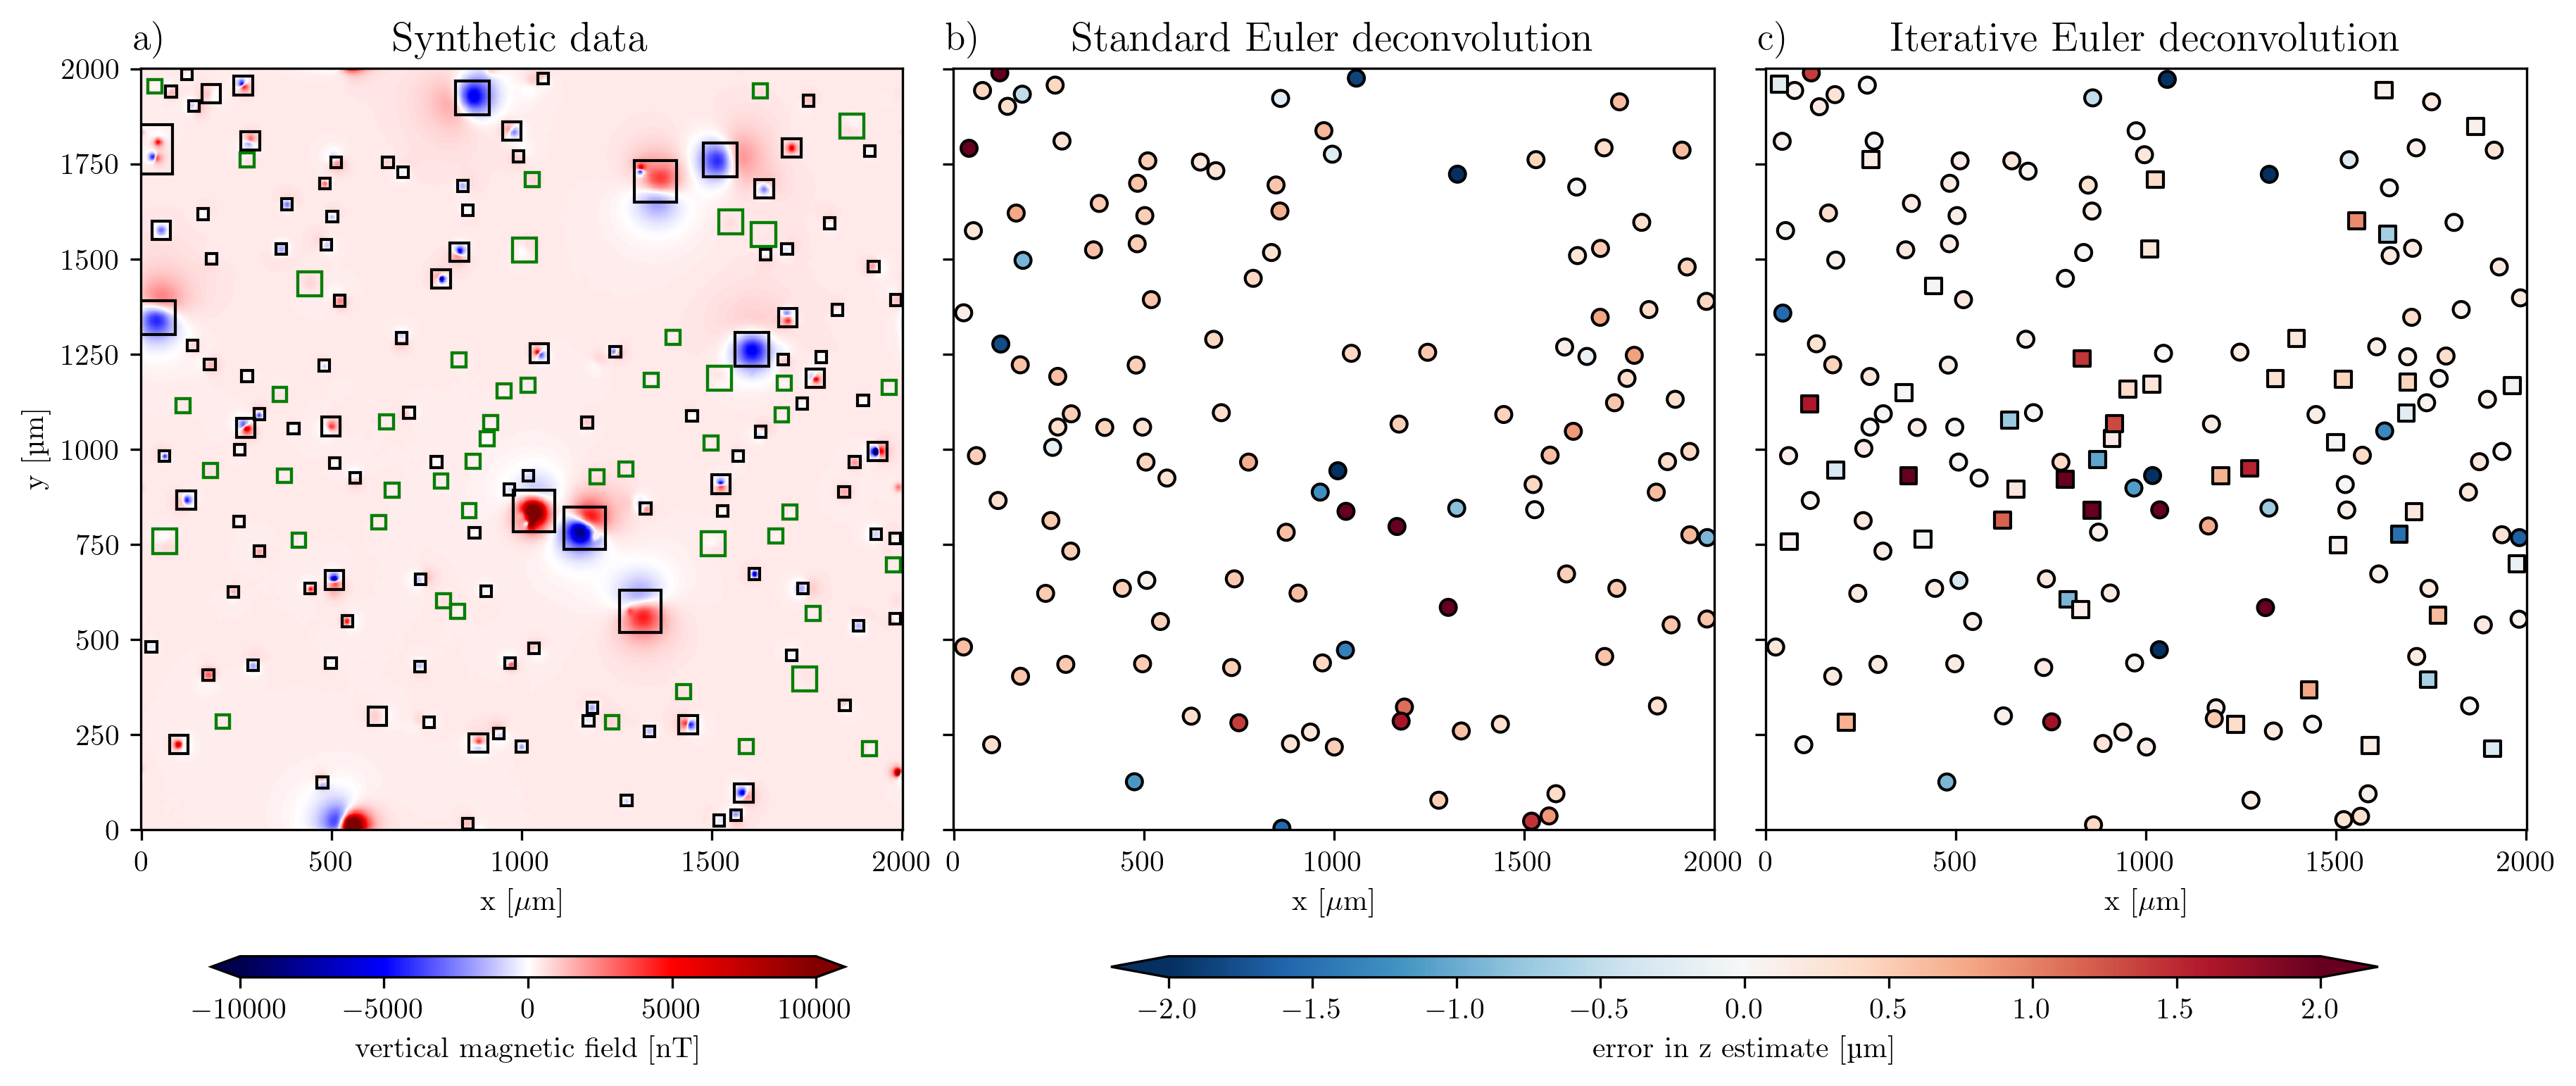
\includegraphics[width=1\linewidth]{figures/euler-comparion-synthetic.png}
  \caption{
    Position estimation for the overlapping signals synthetic sample. (a) Initial detection window data for each magnetic source (black squares) and re-detection provided by the iterative solution (green squares). These data windows were used for the 3D position estimation of magnetic sources (colored circles) in the standard (b) and iterative (c) methodologies. Newly detected sources in the iterative method are represented as colored squares in panel (c).
  }
  \label{euler2}
\end{figure}

The iterative Euler estimated positions were used in the iterative magnetic inversion due to their superior accuracy. In contrast, the standard method relied on positions obtained from the original, unmodified algorithm. Figure~\ref{inversion2} presents a comparison of the estimated magnetic moment directions for the standard (Figure~\ref{inversion2}b) and iterative (Figure~\ref{inversion2}c) methods, in relation to the true directions (Figure~\ref{inversion2}a). As expected, the iterative method provides a better overall agreement with the true directions, recovering a larger number of sources with reliable estimates. The improvement is particularly noticeable as the iterative approach is capable of identifying signals from weaker particles, increasing the number of recovered sources. This has the potential to improve the statistical robustness of the estimated directions, making the method particularly useful for applications in magnetic microscopy.


\begin{figure}[tb!]
  \centering
  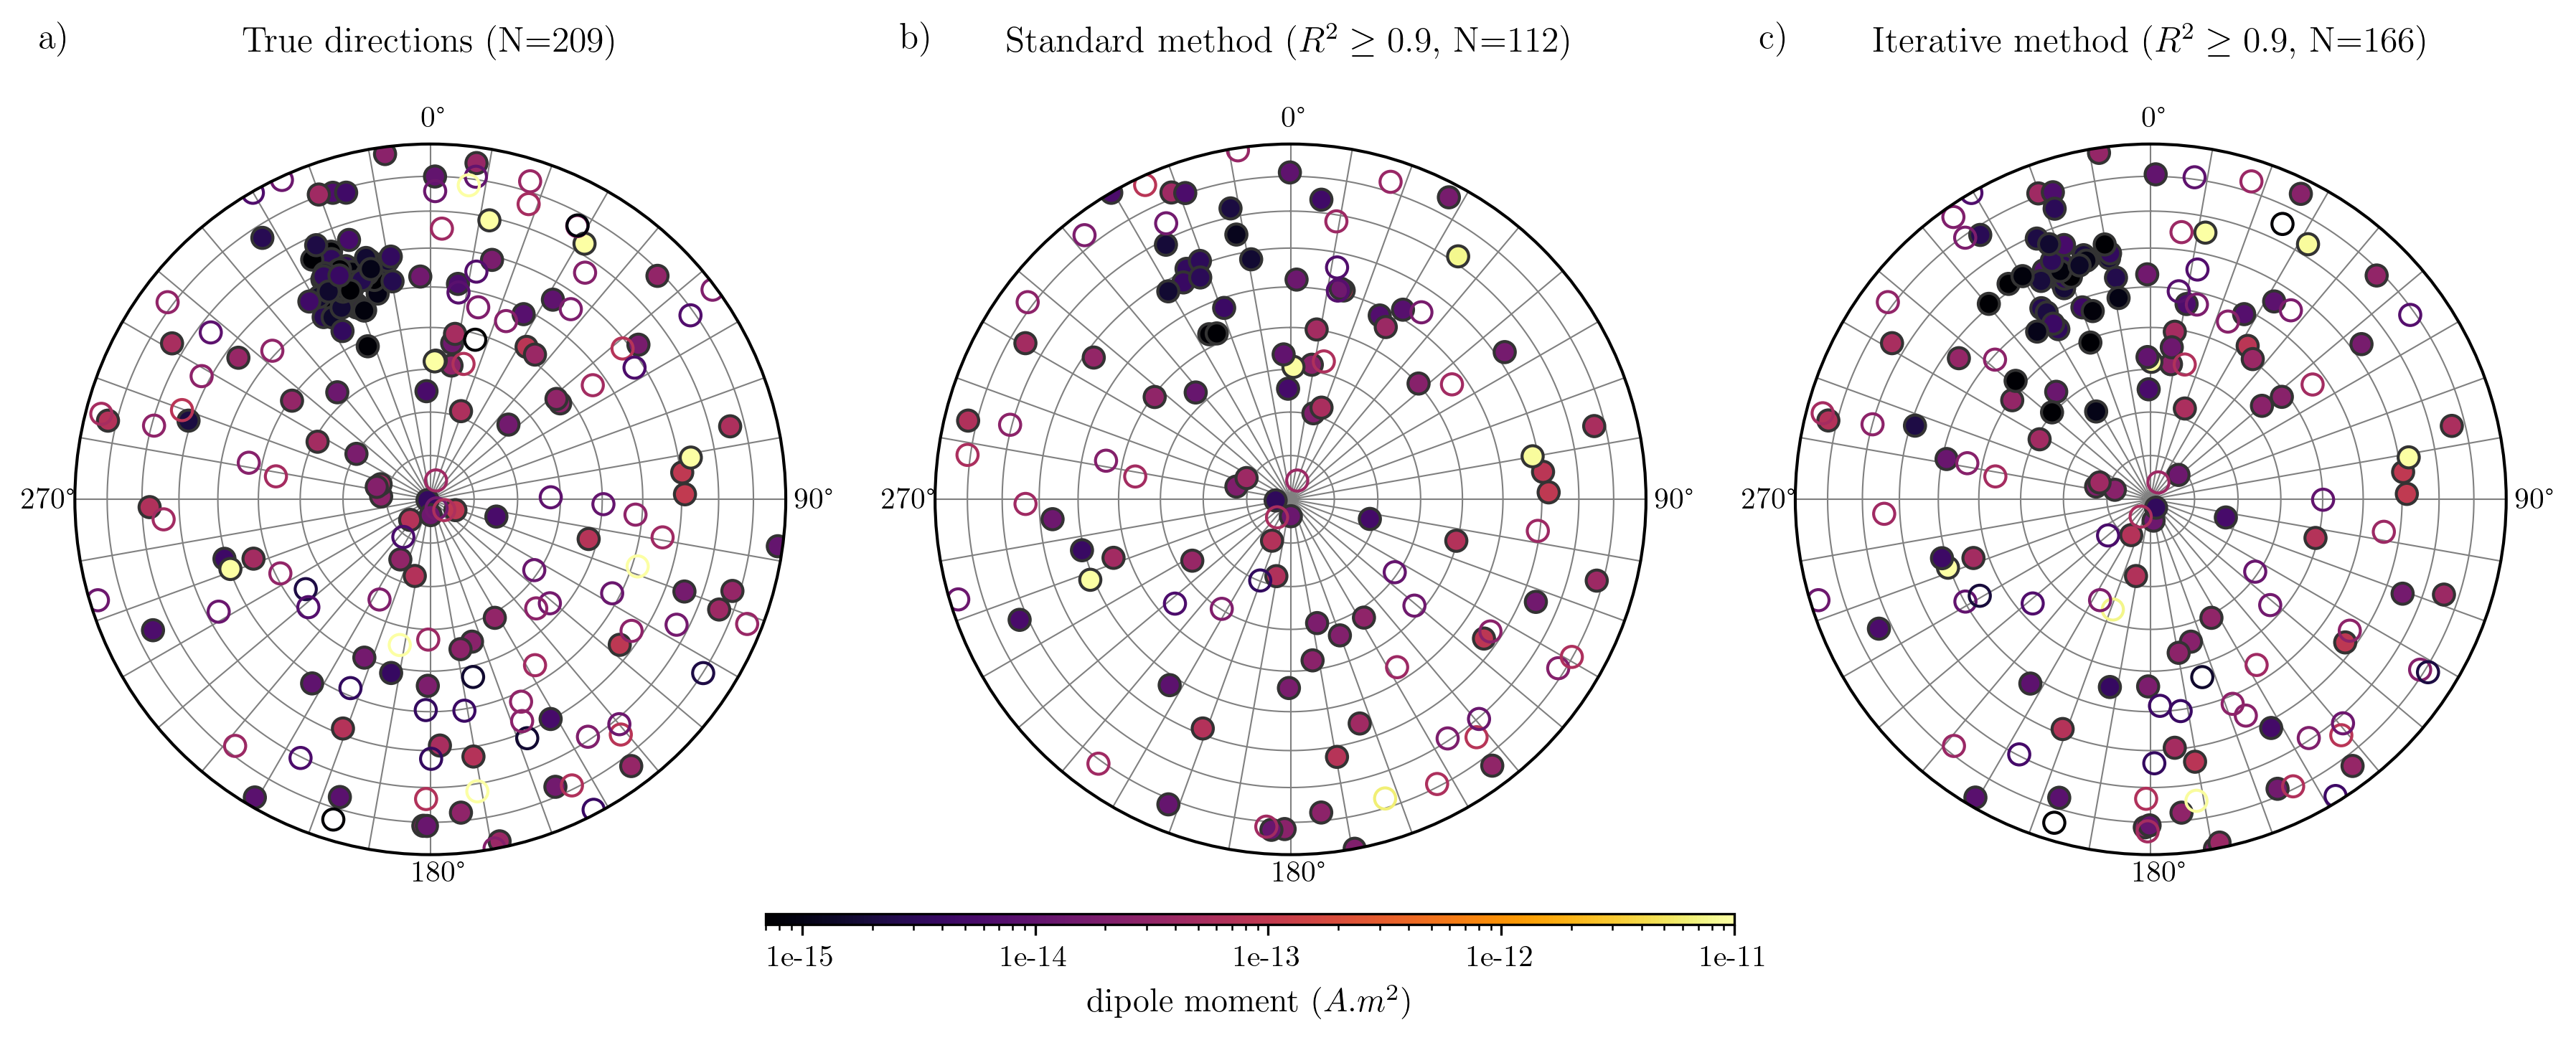
\includegraphics[width=1\linewidth]{figures/synthetic-data-stereograms-comparison.png}
  \caption{
    Comparison of true and estimated dipole magnetic moments and directions for the overlapping signals in the synthetic sample. Panel (a) shows the true modeled direction, while panels (b) and (c) display the estimated vector directions obtained using the standard ($M = 112$) and iterative ($M = 166$) methods, respectively. Results for both methods were filtered based on the coefficient of determination ($R^2 \geq 0.9$). Directions are hued by magnitude of their magnetic moments. Open/closed circles indicate positive/negative inclinations.
  }
  \label{inversion2}
\end{figure}



\subsection{Assessing performance with variable particle density}

To evaluate the influence of particle density on the simulation results, we considered three different grain distributions with \(N = 500\) and \(N = 2500\), corresponding to grain densities of approximately \(9000\) and \(45000\,\mathrm{grains/mm^3}\), respectively. Examples of these distributions are shown in Figures~\ref{synthetic-data-maps}a,b. These densities were chosen to numerically simulate the concentrations expected in different rock types. Lower densities are typical of rocks with scarce magnetic grains, such as carbonates, while the highest density approximates rocks with higher particle concentrations, such as basalts.

\begin{figure}[tb!]
  \centering
  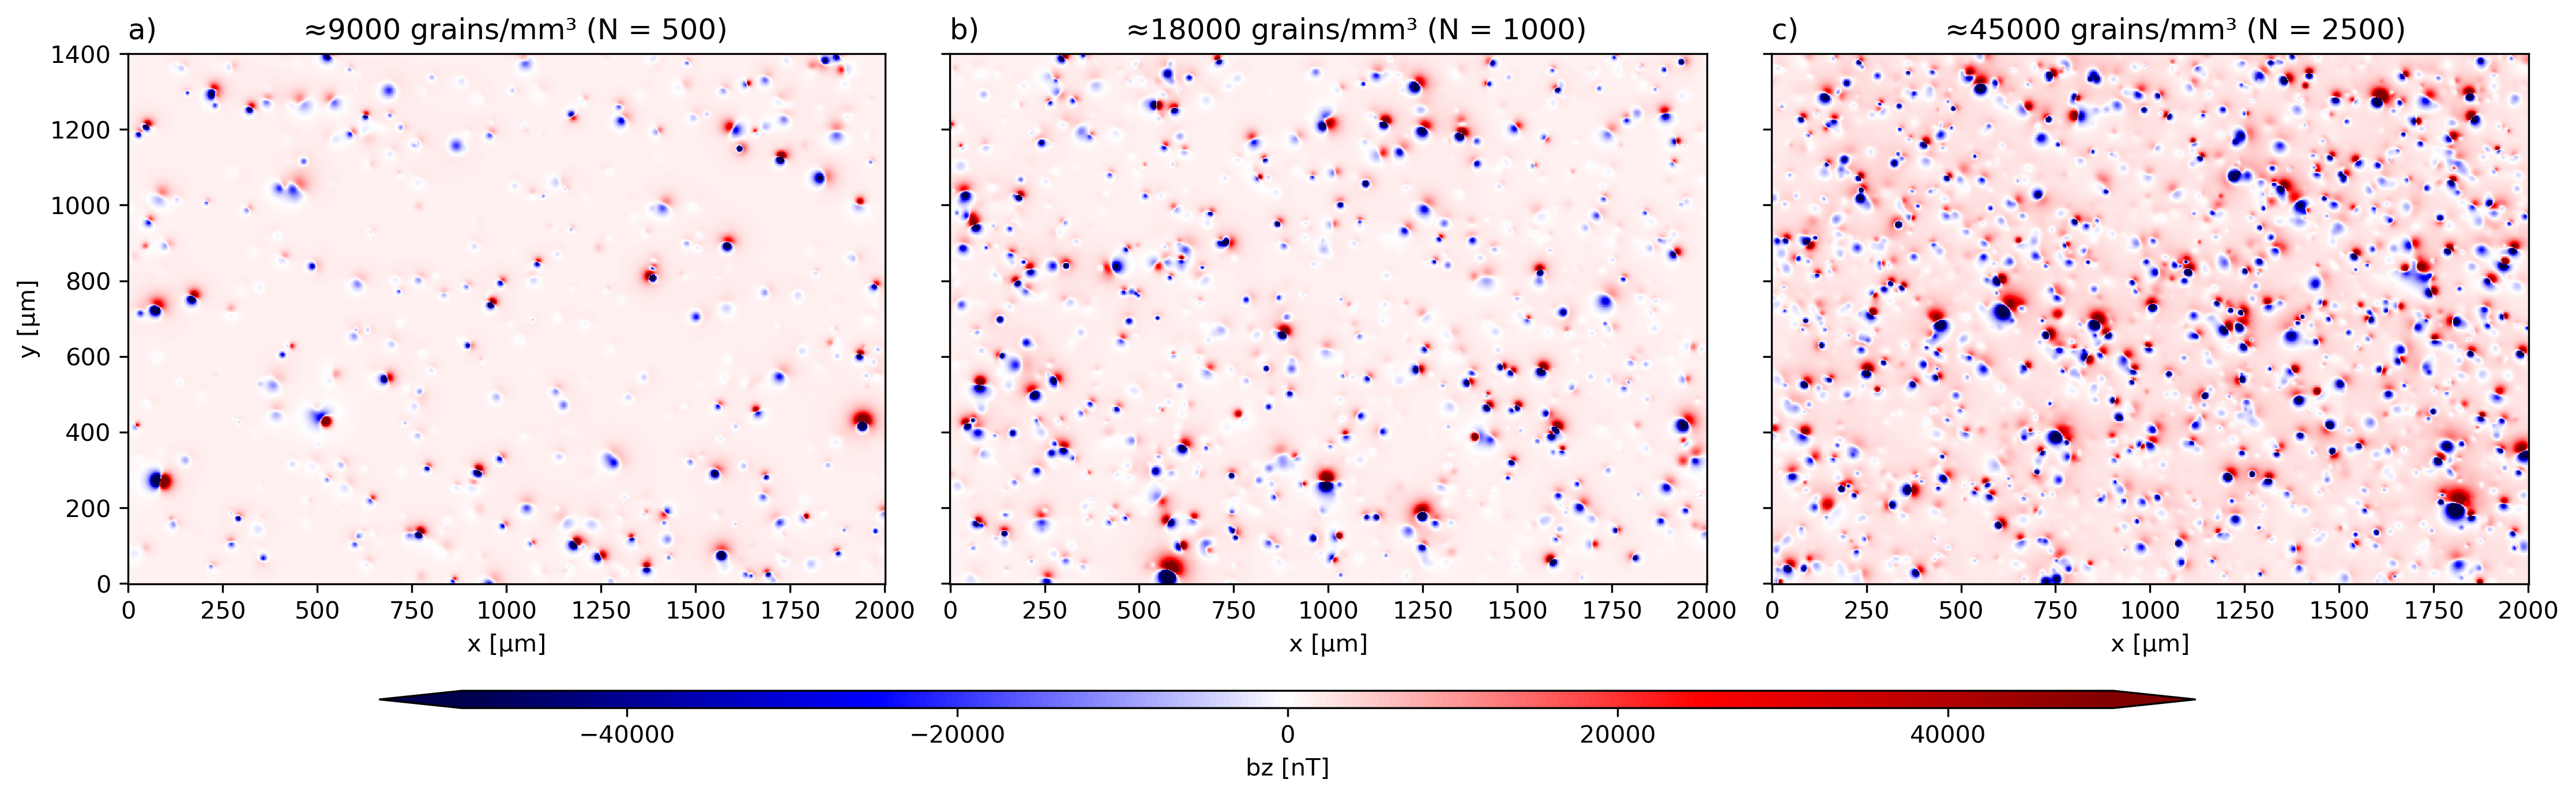
\includegraphics[width=1.0\linewidth]{figures/synthetic-different-densities-maps.png}
  \caption{
Vertical component (\(b_z\)) magnetic data from synthetic grain distributions used to evaluate the influence of particle density on the simulation. Panel (a) shows an example with \(N = 500\), highlighting a low-density distribution of grains. Panel (b) illustrates the distribution for \(N = 1000\), presenting a moderate density of grains. Panel (c) displays the distribution for \(N = 2500\), showing a high-density grain arrangement.
  }
  \label{synthetic-data-maps}
\end{figure}


The directional parameters and magnetic moment intensities distributions were kept constant across all simulations, as the goal was to isolate the effects of increasing particle density. For each simulation, the total \(N\) magnetic dipole sources were created and randomly distributed across a thin section of \qty{2000}{\um} \(\times\) \qty{1400}{\um}. The dipole moments were sampled from a lognormal distribution centered at a mean amplitude of \(1 \times 10^{-14}\,\mathrm{A \cdot m^2}\), with a standard deviation spanning two orders of magnitude. This configuration ensures that most of the distribution is concentrated around the mean, while also allowing for the presence of particles with magnetic moments as strong as \(10^{-11}\,\mathrm{A \cdot m^2}\), simulating larger particles with a greater influence on the magnetic field compared to weaker particles. The modeled sources were also positioned at pseudo-random depths ranging from 1 to \(\qty{20}{\micro\meter}\).

A variety of geological processes can lead to the acquisition of natural remanent magnetization (NRM). If the NRM is primary—acquired at the same time as the rock—it will generally align with the ambient magnetic field, such as a planetary field. However, the alignment of individual grains is influenced by multiple factors, including particle properties \citep[shape, size, domain state,][]{Bellon2025} and the conditions under which NRM is acquired, such as the cooling rate of lavas. As a result, while individual grain signals may show a general tendency toward alignment, the magnetic moments of many particles will still exhibit some degree of random orientation. However, modeling TRM directions is not a straight-forward task, instead we can mirror an isothermal remanent magnetization (IRM) behavior in our synthetic data. Thus by setting the inclination and declination of directional parameters primarily at 30° and 330°, respectively, and 50° dispersion angle introduced variability within spherical statistics, where directional data extends over a unit sphere rather than Cartesian coordinates. This angle indicates a broad spread of directions around the mean, accounting for significant variability in dipole directions, which is crucial for accurately representing the natural diversity of magnetic sources.

The synthetic magnetic field \(b_z\) was computed over a grid with a \qty{2}{\um} spacing, and the measurement plane was set at a constant height of \qty{5}{\um} above the thin section. The same high-frequency QDM spatially correlated pseudo-random noise was added to the computed field to mimic realistic measurement conditions. Additionally, a positive baseline shift of \(\qty{400}{\nano\tesla}\) \citep[following][]{Hess2024} was introduced to replicate the acquisition process in magnetic microscopy. The simulations were conducted in a zero external field environment, where all signals generated in the maps were solely and exclusively caused by the magnetization of the simulated particles, simulating real acquisitions typically performed in magnetically shielded rooms to eliminate the influence of the Earth's geomagnetic field. A total of 10 simulations were carried out for each different particle density level.

The results reveal a clear difference in the performance of the standard (red curves and left stereoplots) and iterative (blue curves and right stereoplots) methods in reconstructing the synthetic IRM direction imparted in the simulations. As shown in Figure~\ref{synthetic-data-stereograms}a, for lower densities of particles, both methods perform almost the same, given that in this case, the amount of interference between the sources is small. This is also observed for the mid-term density (Figure~\ref{synthetic-data-stereograms}b). However, for the higher density of magnetic particles (Figure~\ref{synthetic-data-stereograms}c), the iterative method starts to outperform the standard method. This shows the superiority of the iterative technique, as there are no randomly stronger particles simulating different viscous directions. Even though there are many strong sources, they all follow the same distribution around the synthetic direction, similar to what happens in an IRM induced sample. This could explain, alongside the low density of particles, the good results presented by the real carbonatic data presented by \citet{Souza-Junior2024}, which was subjected to strong IRM, though it remains ambiguous whether the results are due to the low particle density or the IRM. For this reason, the next tests involved samples with natural remanent magnetization.

\begin{figure}[tb!]
  \centering
  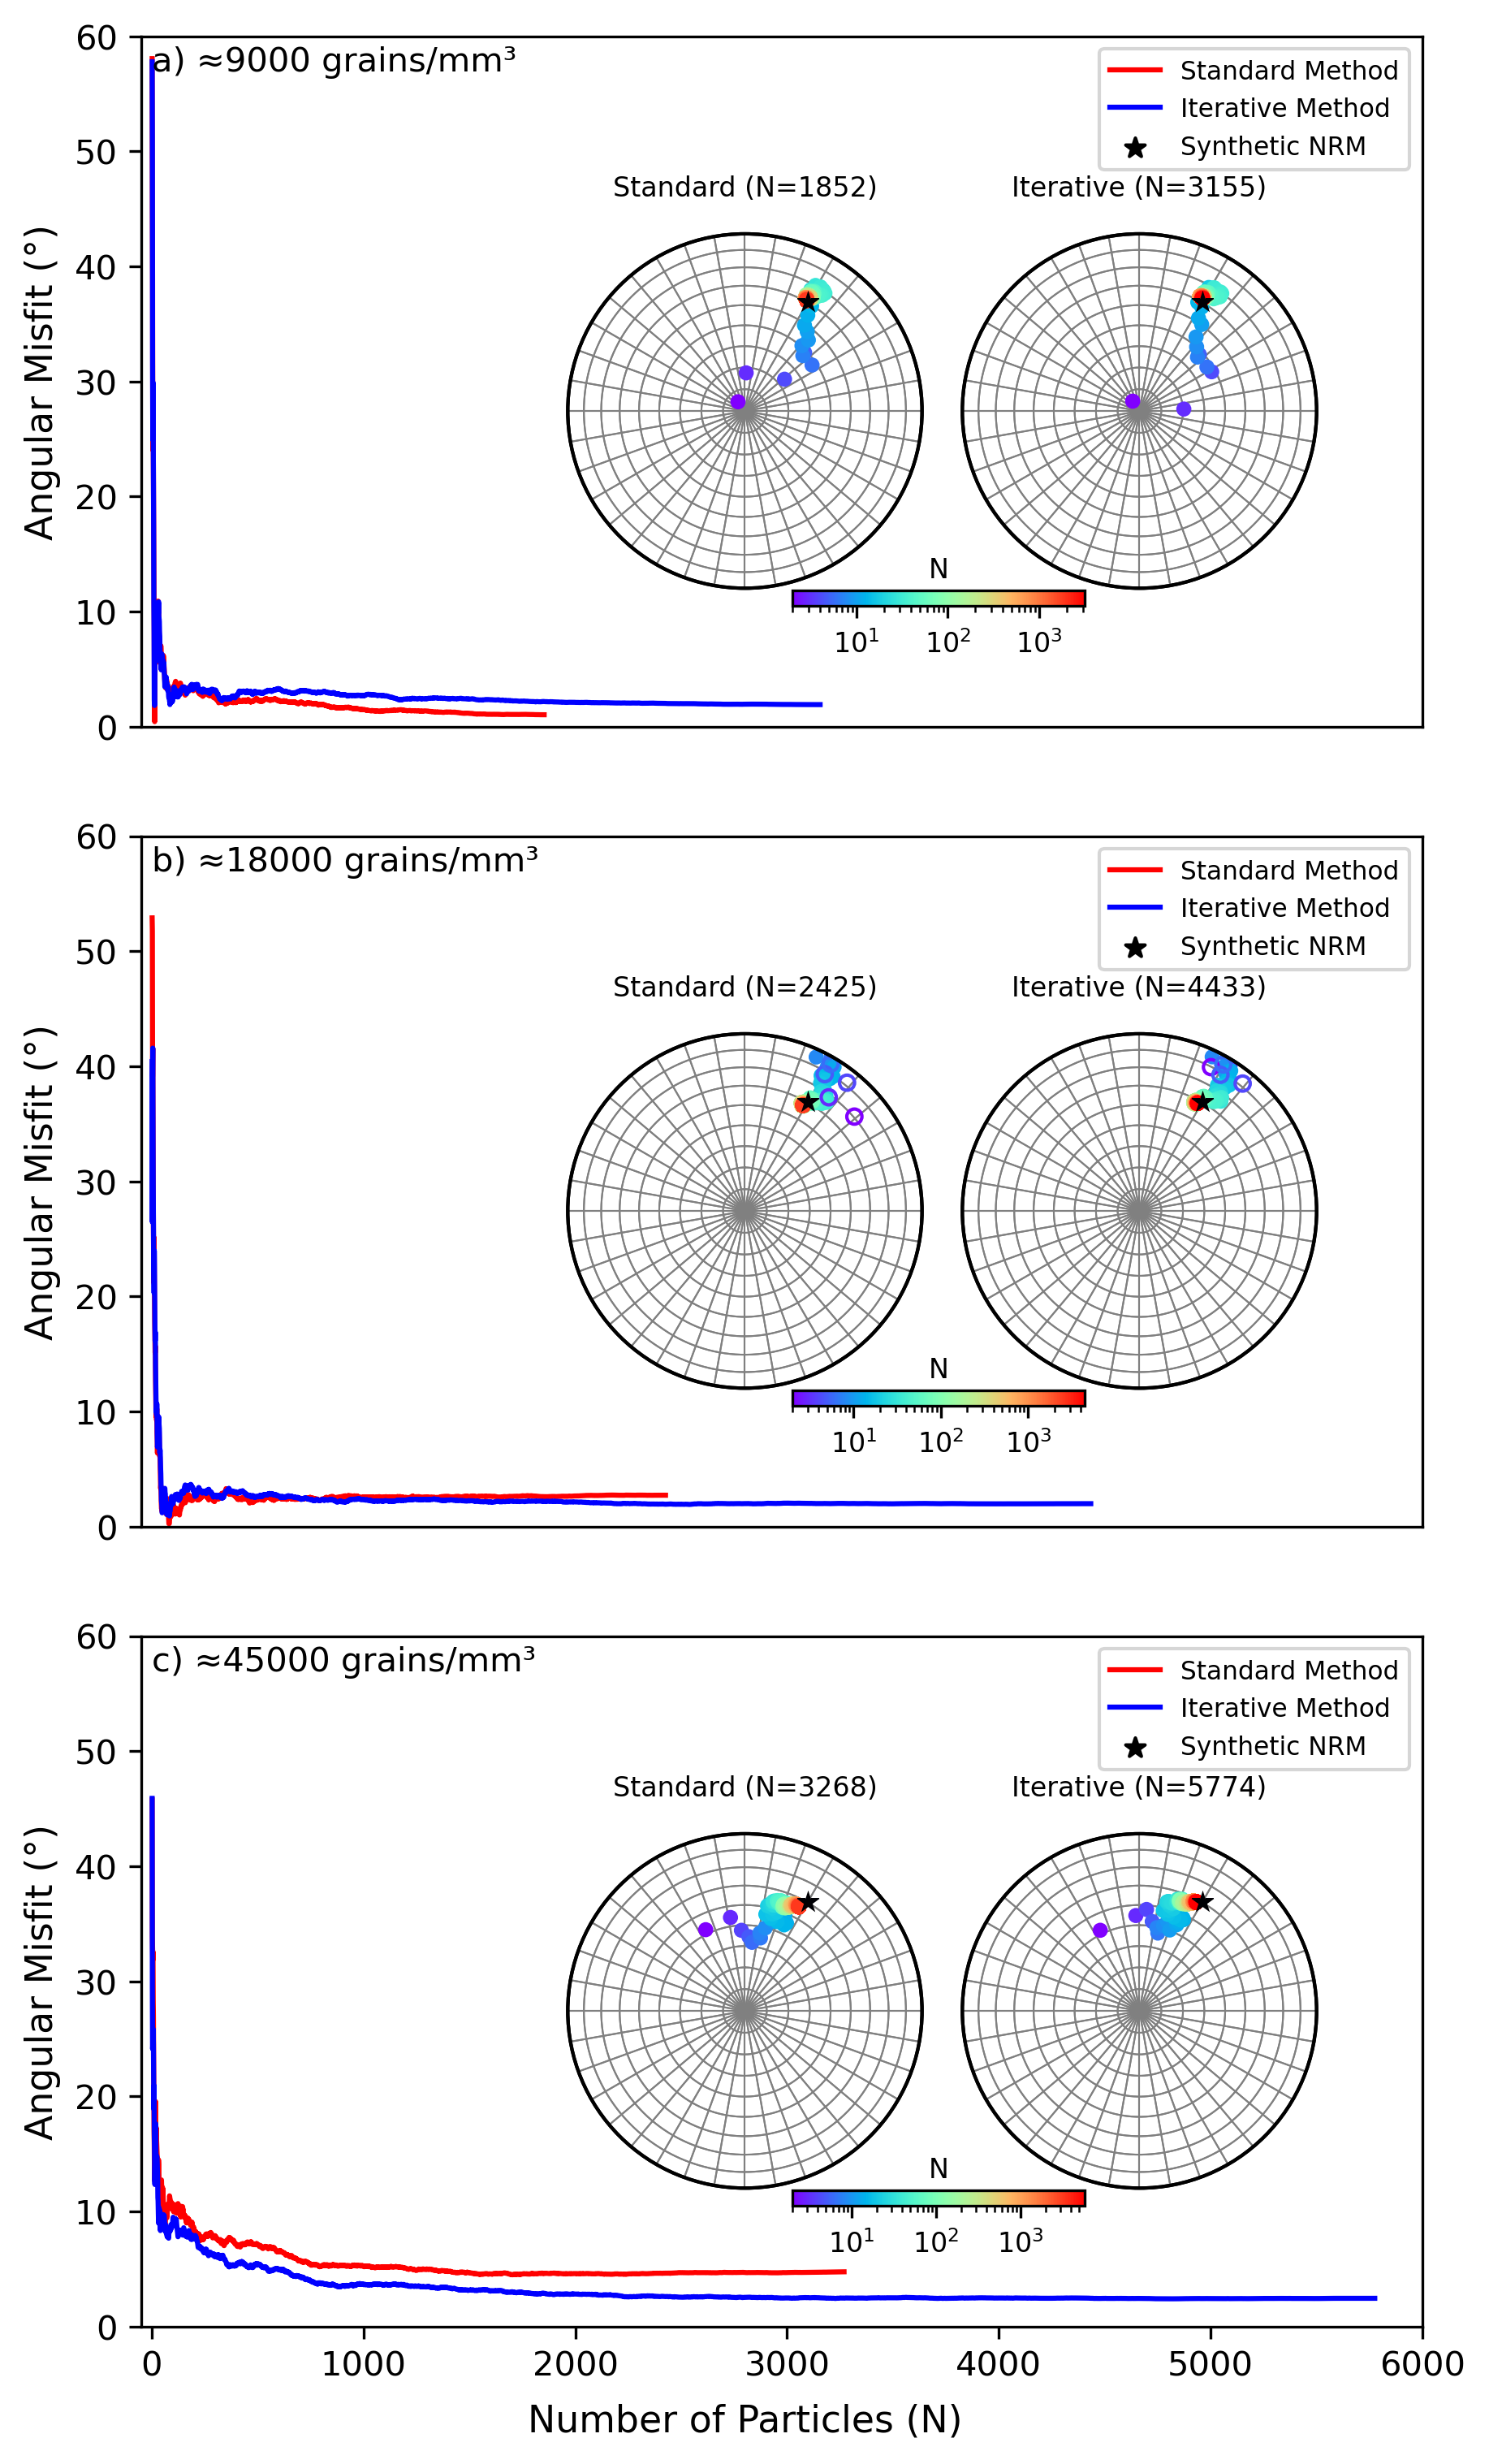
\includegraphics[width=1.0\linewidth]{figures/synthetic-different-densities-stereoplot.png}
  \caption{
Comparison of the magnetic directions obtained using the original (red line and left stereogram) and the iterative (blue line and right stereogram) methods on each synthetic grain distributions simulation. Panel (a) shows the angular misfit between the cumulative vector and the measured magnetic direction for the low-density distribution. Panel (b) illustrates the angular misfit for the moderate-density distribution. Finally, panel (c) presents the results for high-density distribution. The stereographic projections of the filtered magnetic vectors ($R^2 \geq 0.9$) for each density are also shown, with modeled bias direction (star) and the cumulative direction (square) indicated. The color gradient represents the logarithmic scale of particle counts, with warmer colors indicating higher particle concentrations.
  }
  \label{synthetic-data-stereograms}
\end{figure}


\section{Real data applications}

After demonstrating the applicability of the new methodology through the numerical simulations, we applied it to real MM data. The magnetic particles \citep[most commonly magnetite,][]{OReilly1984} acquire TRM as they cool below their Curie temperature, with the magnetization direction becoming "locked in" upon reaching the blocking temperature \citep{Dunlop1997}. When grains are sufficiently small and exhibit homogeneous, unidirectional magnetization (single domain, SD), the acquisition and preservation of magnetic signals are physically described by Néel’s theory \citep{Neel1949, Neel1955}. This allows them to retain remanent magnetization for billions of years, making them excellent recorders of the paleomagnetic field. In addition to SD particles, pseudo-single domain (PSD) particles—characterized by flower and vortex states—are also stable and can preserve magnetization for timescales comparable to the age of the Solar System \citep{Nagy2017, Lascu2018,Bellon-2024a}. Conversely, Néel’s theory does not apply to larger particles (multidomain, MD), which have unstable remanent magnetization \citep[e.g., due to viscous domain reorganization,][]{DeGroot2014}, limiting their capacity to reliably record the geomagnetic field.

In this section, we worked with two distinct samples. The NRM of these samples was measured using the 2G RAPID Superconducting Rock Magnetometer at the Harvard Paleomagnetics Lab, Department of Earth and Planetary Sciences, Harvard University. As a result, the measurements encompass both the primary TRM and any possible viscous components acquired through the natural magnetic relaxation of some particles. Additionally, to ensure consistency between the magnetometer measurements, which were taken vertically, and the maps produced with the QDM, it was necessary to apply a 90-degree clockwise rotation around the \textit{x}-axis to the vertical measurements. This rotation ensures that both measurements are in the same reference frame.

The samples we used provide test to:

\begin{enumerate}
\item \textbf{Evaluate a stable, dispersed assembly:} The first test focuses on the analysis of a thin section made of an archaeological ceramic (Figure~\ref{real-data-maps}a). This sample is characterized by a moderate density of magnetic particles, most falling into SD and PSD categories. The goal of this test is to assess the method’s performance in real samples where the magnetic carriers are stable, and the influence of unstable domains is minimal. This setting allows for a clear evaluation of the methodology’s sensitivity and accuracy when working with well-defined magnetic signals.

\item \textbf{Evaluate a Complex Densely Packed Assembly:} The second test involves the examination of the basaltic rock sample (Figure~\ref{real-data-maps}b). This sample acquired its TRM during the natural cooling of mafic lava, leading to a high density of magnetic particles. Unlike the ceramic sample, the basalt is significantly influenced by unstable MD particles, which introduce additional complexity to the magnetic signal. The aim of this test is to verify the method’s effectiveness in identifying and analyzing magnetic sources in challenging conditions, where densely packed magnetic carriers and the presence of unstable remanent magnetization could affect the reliability of the results. This is a more complex and challenging scenario, providing a test for the accuracy of the method to identify and interpret magnetic sources in samples with densely packed and less stable magnetic carriers.
\end{enumerate}

\begin{figure}[tb!]
  \centering
  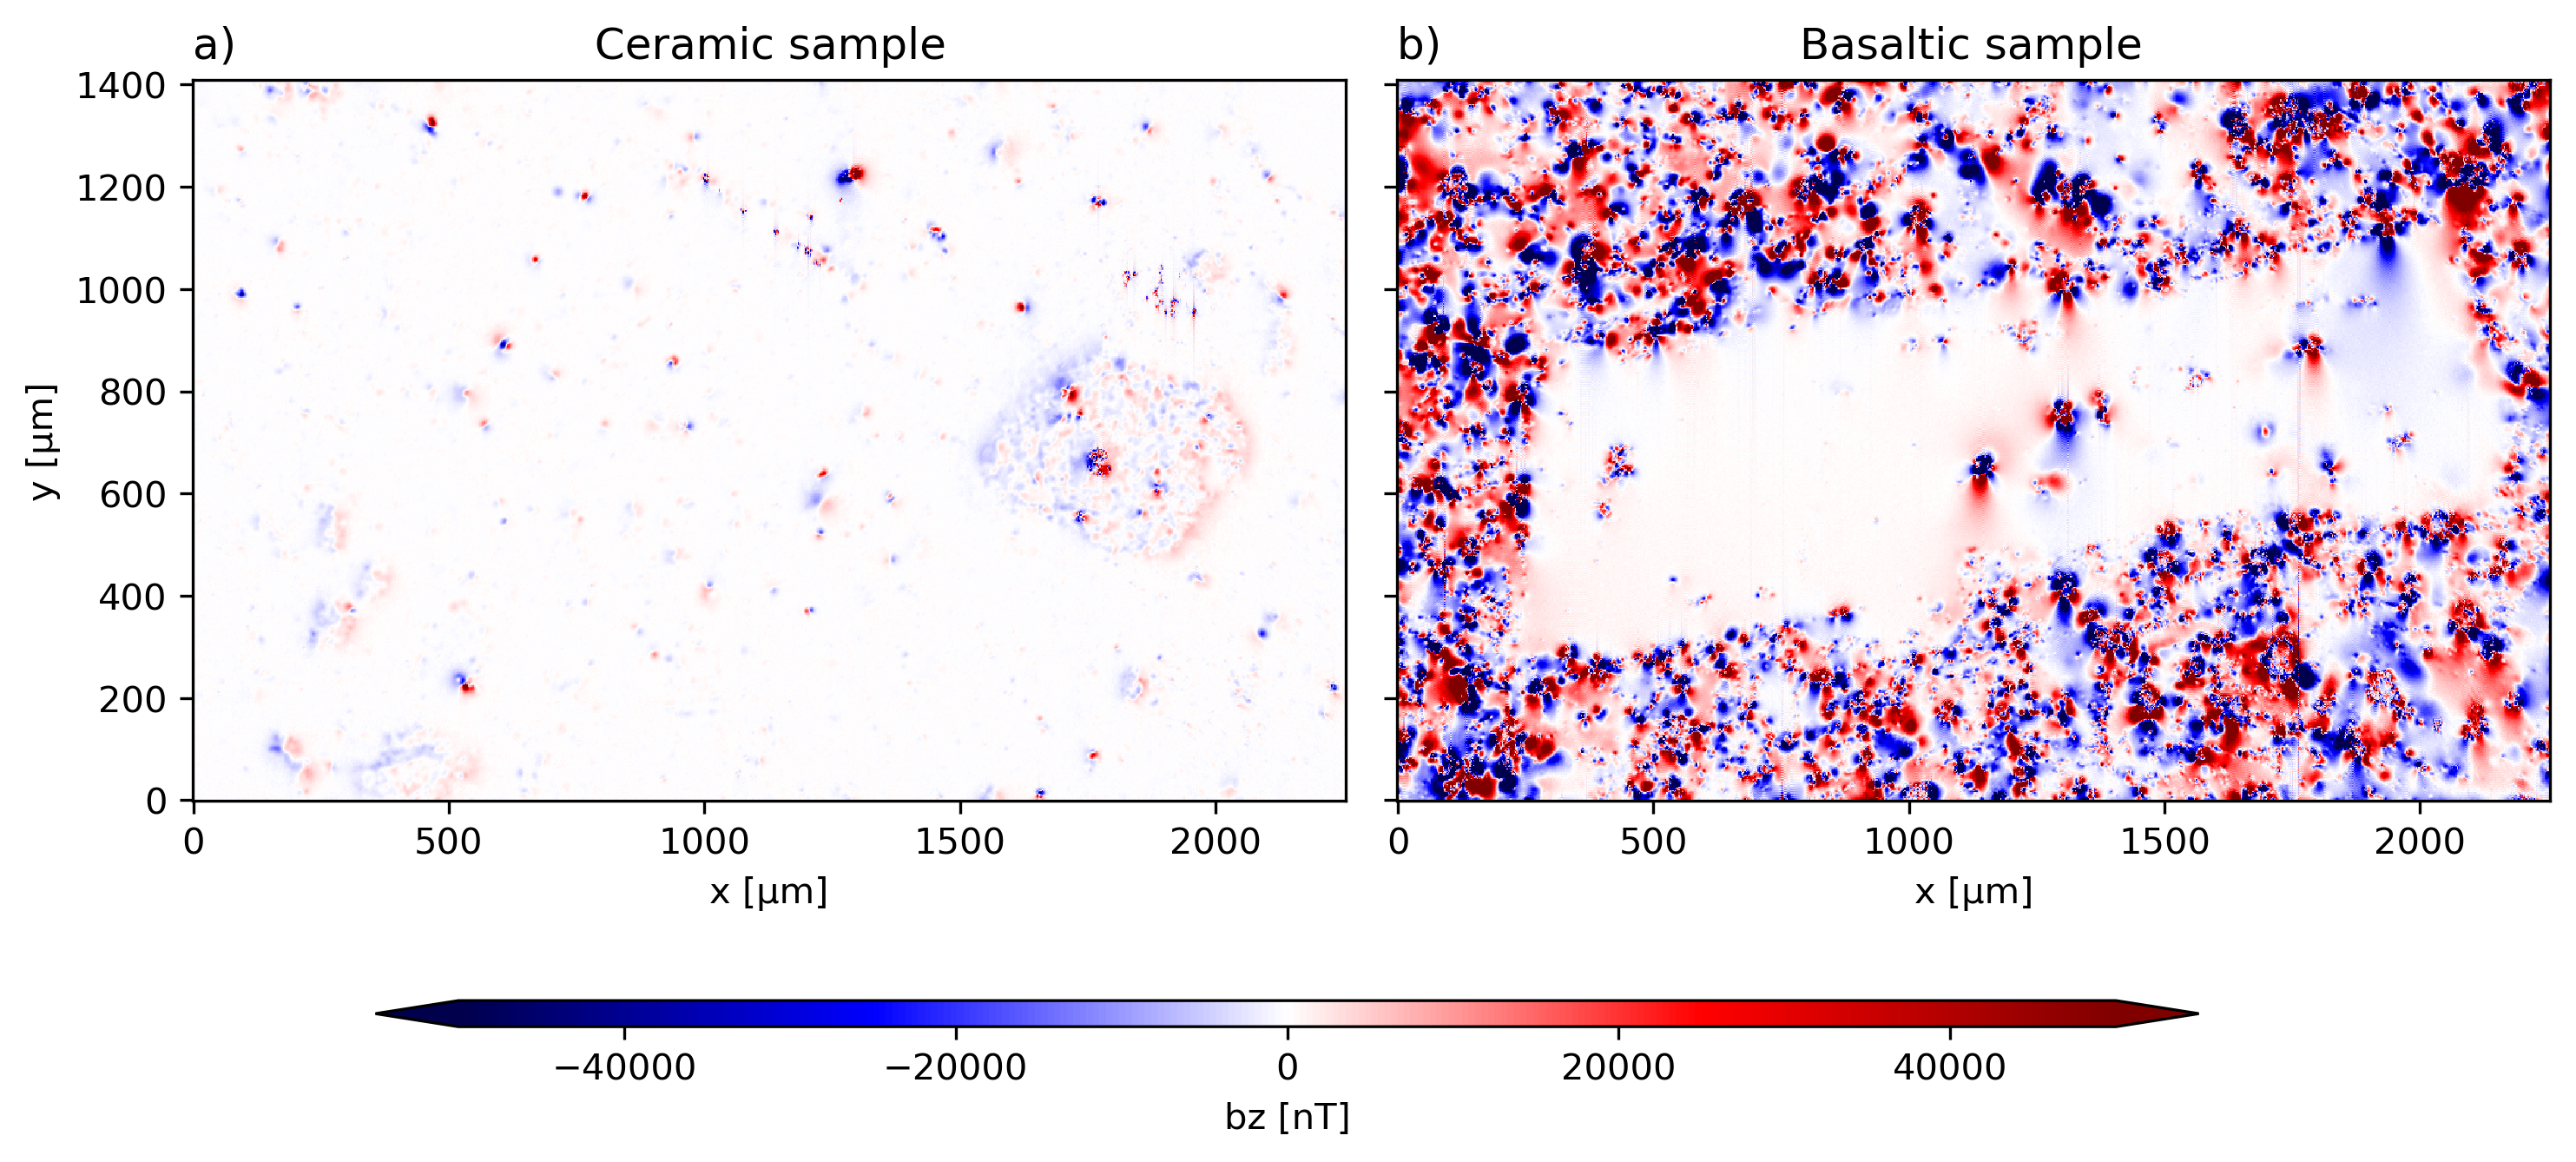
\includegraphics[width=1\linewidth]{figures/real-data-maps.png}
  \caption{
   LED picture (left) and vertical component (\(b_z\), right) magnetic data from real samples observed at \(z = 5\) µm. Panel (a) shows an example from the ceramic tile sample, highlighting its key characteristics, including the presence of isolated dipolar particle signals and clusters related to larger particles. Panel (b) presents an example from the basaltic sample, displaying two main occurrences of magnetic signals: the first is a high density of signals distributed within the matrix, and the second appears as inclusions in plagioclase phenocrysts.
  }
  \label{real-data-maps}
\end{figure}

\subsection{Evaluation with a stable, dispersed assembly}

To evaluate the feasibility of magnetic microscopy techniques in detecting and characterizing TRM, we selected a well-preserved fragment of baked clay pavement tile (sample RSLG1) from the archaeological site São Luiz Gonzaga reduction (1657-1687 AD). This fragment was studied by \citet{Poletti2016}. According to these authors, the magnetic properties of the sample indicate that magnetization is carried by a low-coercivity phase, most likely PSD Ti-poor titanomagnetite. Their interpretation is supported by the IRM curves saturated at fields up to approximately 0.3 T, narrow hysteresis loops, and maximum NRM demagnetization temperatures around 550°C. First order reversal curves (FORC) also confirm a predominance of non-interacting SD/PSD grains. These characteristics make the sample an ideal candidate for magnetic microscopy studies aimed at investigating its natural remanent magnetization.

We mapped the NRM of the thin-section sample using the QDM at the Harvard Paleomagnetics Lab, Department of Earth and Planetary Sciences, Harvard University. All QDM data were taken in projected magnetic microscopy (PMM) mode and converted to the vertical component of the magnetic field ($b_z$) using a spectral approach \citep{Fu2020, Glenn2017, Lima2009}. We applied a 0.9 mT bias magnetic field during measurement, which was reversed periodically to result in a net bias field of ~400 nT. A total of 20 randomly selected regions were subjected to this procedure to ensure representative coverage of the sample's magnetic properties, in which Figure~\ref{real-data-maps}a showcases one of the maps obtained. The scanned area measured $\qty{1410}{\um} \times \qty{2256}{\um}$ with a grid spacing of \qty{2.35}{\um} ($N = 576 \times 10^{3}$). Data acquisition was conducted at a constant sensor-sample distance of \qty{1} - \qty{5}{\um}. This allowed for high-resolution mapping of the magnetic field distribution.

We have applied both the standard and iterative algorithms to this data, and all magnetic vectors associated with the identified particles were compiled into a database. This dataset was filtered based on the model's coefficient of determination ($R^2$), with only vectors meeting the criterion of $R^2 \geq 0.9$ being retained. This filtering is important to remove inversion results that do not comply with our dipolar assumption. An $R^2 \geq 0.9$ means that the only results that closely fit the data are kept (the maximum value of $R^2$ is 1).  The selected vectors were then ordered by intensity and progressively summed. At each step, the cumulative vector was compared with the NRM measured of the whole sample (which was acquired with a 2G Superconducting Rock Magnetometer, see the Methodology section for more details).

The comparison between the standard and iterative algorithms highlights significant differences in their ability to reconstruct the NRM of the sample. As shown in Figure~\ref{ceramic-data-stereograms}, the angular misfit between the cumulative magnetic vector and the measured NRM decreases more effectively with the iterative approach. We further remove outliers in the dataset by excluding values that are 1.5 times larger than the third-quartile of the dipole moment intensities. While the non-filtered standard method results in a consistently higher misfit, stabilizing around \ang{55}, the iterative method quickly refines the alignment, reducing the misfit to approximately \ang{10} within a few hundred particles. While for filtered curves this misfit difference reduces, there are virtually no changes in the iterative method result. This indicates that the iterative approach is more efficient in capturing the true remanent magnetization with fewer contributing grains. The stereographic projections further support this observation by illustrating the directional distribution of the filtered vectors for each method, where the iterative approach yields a distribution more closely aligned with the measured NRM (star symbol) and the cumulative direction (square symbol). These results demonstrate that the iterative method significantly enhances the accuracy of NRM reconstruction by effectively mitigating directional dispersion.

The limited improvement threshold in directional accuracy, even as more particles are added, is a noteworthy observation. We propose two possible contributing factors. First, as previously discussed, the bias of individual particles towards the magnetic field is only at the level of $\sim1\%$. When measuring the total NRM at the macroscopic scale, the contributions of all grains are summed, allowing randomly oriented signals to cancel out while the more aligned grains enhance the overall alignment with the field direction. Classical rock thin sections, like the one used in this study, are typically prepared at a thickness of around \qty{30}{\um} to facilitate the identification of mineral features under a petrographic microscope. Within such a thin section, millions of magnetic minerals are likely present. However, in MM data acquisition, we only sample a small portion of the entire thin section. Even within this measured area, not all magnetic signals are fully detected, as the measured magnetic moment depends on both the depth of the particles and their magnetic strength. As a result, when more particle directions are incorporated into the combined magnetic signal, a saturation effect may occur. Beyond a certain threshold, the inclusion of additional, randomly oriented signals could outweigh the contribution of well-aligned grains, limiting further improvement in directional accuracy. This would explain why, despite increasing the number of particles, the expected refinement in the reconstructed direction is not observed.

The second hypothesis involves human-induced errors during the measurement process. The sample had to be manually positioned and oriented in both the QDM and the 2G magnetometer, introducing potential sources of misalignment. In the 2G magnetometer, the sample was measured in a vertical orientation and later rotated to match the reference frame of the thin section used in the QDM analysis. This manual handling and reorientation may have introduced small but cumulative misalignments, contributing to the observed directional discrepancies. Another potential source of bias in the 2G magnetometer measurements could be contamination, either from the glass slide or another external source near the sample.

\begin{figure}[tb!]
  \centering
  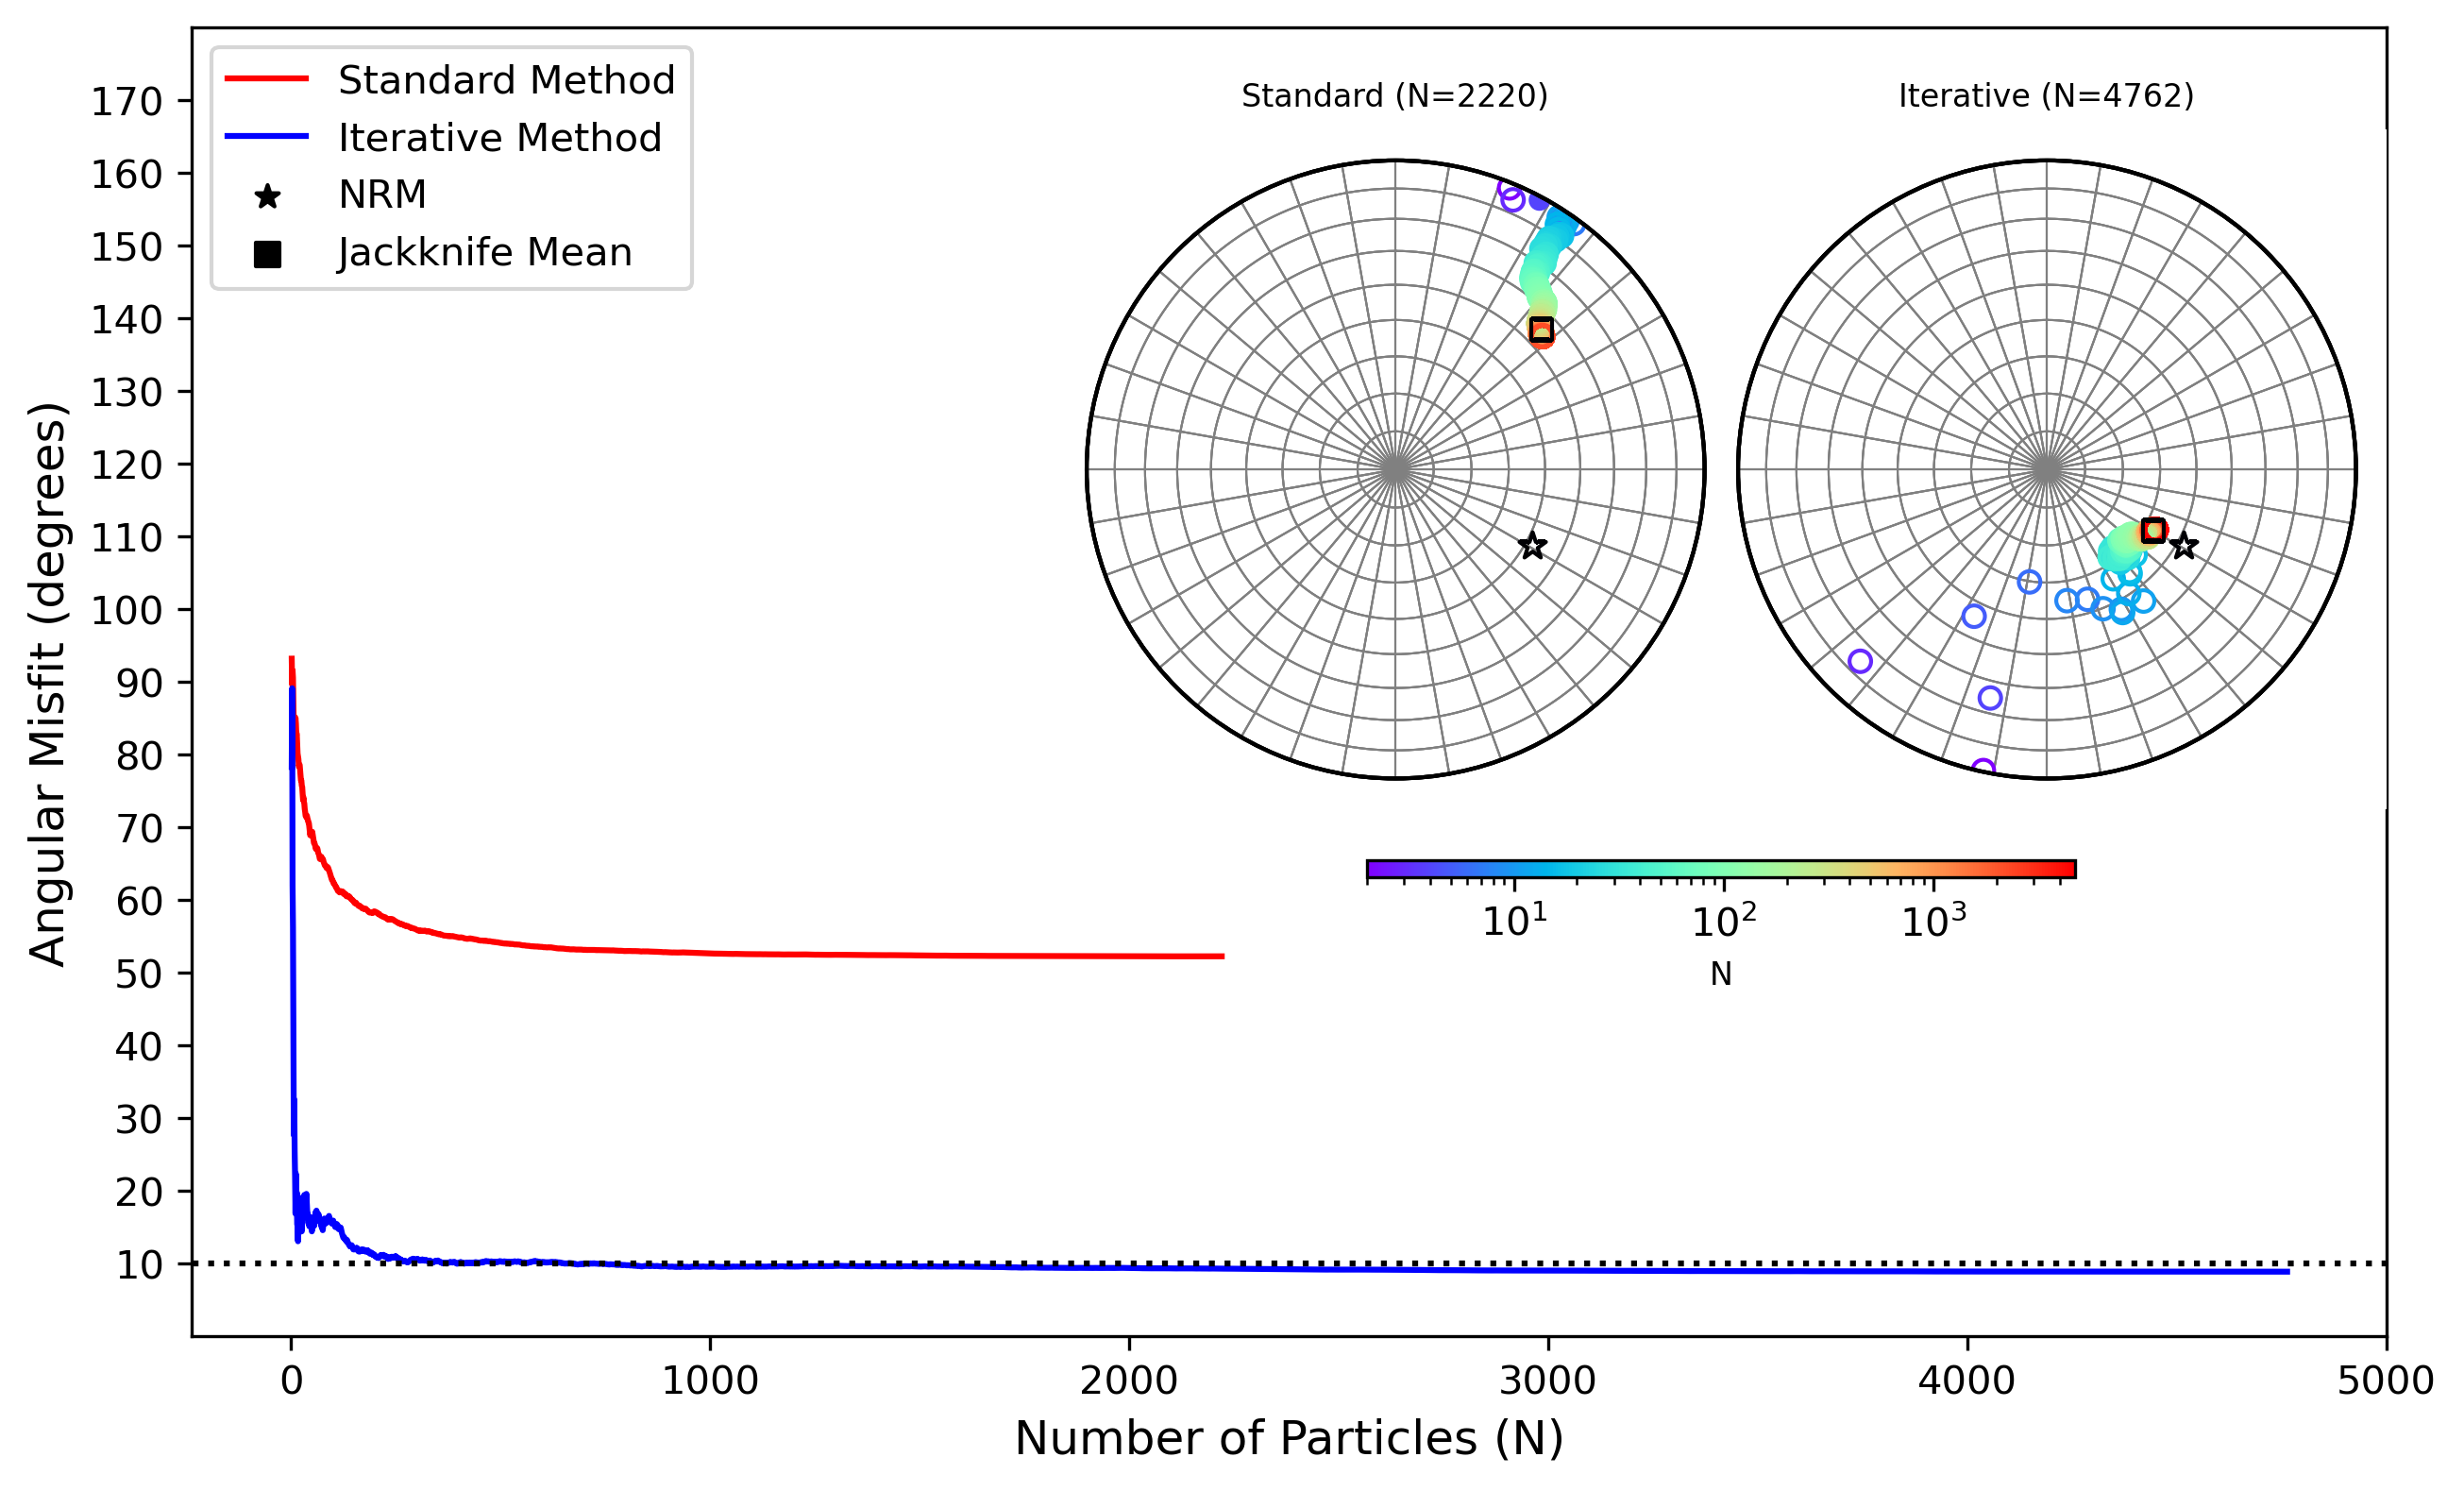
\includegraphics[width=1\linewidth]{figures/ceramic-data-stereoplot.png}
  \caption{
  Comparison of the standard (red) and iterative (blue) algorithms in reconstructing the NRM direction from the ceramic sample. (Left) Angular misfit between the cumulative vector and the measured NRM as a function of the number of particles ($N$). (Right) Stereographic projections of the filtered magnetic vectors ($R^2 \geq 0.9$) for both methods, with the measured NRM (star), non-filtered cumulative direction (triangle), and the filtered cumulative direction (square) indicated. The color gradient denotes the logarithmic scale of particle counts, with warmer colors representing higher concentrations. The solid-lined and dashed-lined curves represent the non-filtered and outliers filtered data, respectively.
  }
  \label{ceramic-data-stereograms}
\end{figure}

%%%%%%%%%%%%%%%%%%%%%%%%%%%%%%%%%%%%%%%%%%%%%%%%%%%%%%%%%%%%%%%%%%%%%%%%%%%%%%%
\subsection{Evaluation with a complex densely packed assembly}

In order to apply our method to a more magnetically complex sample, we have chosen a basalt from the Caviahue-Copahue volcanic complex (Argentina), specifically a core from the Cola de Zorro Formation (COP01) \citep{Moncinhatto2019}. This formation exhibits a flow-aligned fabric, marked by plagioclase crystals, but also contains both phenocrysts and smaller crystals in the matrix showing a trachytic texture. Its magnetic mineralogy is mainly composed of low-Ti magnetite, with most macroscopic crystal sizes ranging from 10 to 50 \si{\micro\meter} \citep{Moncinhatto2019}. This size distribution is reflected in the high-field experiments, including IRM acquisition curves, hysteresis loops, and FORC diagrams. They reveal saturation at fields around 0.2 \si{T}, coercivities below 10 \si{mT}, and the FORC diagrams are typical of multidomain (MD) grains. Nonetheless, other samples within the same formation display coercivities between 10 and 20 \si{mT} and FORC diagrams characteristic of magnetite with a PSD behavior, or mixtures of SD and MD grains.

The acquisition of QDM data was essentially the same as the aforementioned experiment with the ceramic tile. The QDM scans were performed to capture the magnetic field distribution at high spatial resolution. To better compare the results with the tile sample, the same number of randomized mapping spots was performed. Figure~\ref{real-data-maps}b shows one example of the maps obtained. The resulting data enabled the calculation of angular misfit as a function of the number of particles, providing insight into the reliability of different analytical methods.

The results reveal a clear difference in the performance of the standard and iterative methods in reconstructing the NRM direction. As shown in Figure~\ref{basalt-data-stereograms}, the iterative method consistently achieves lower angular misfit values, before and after the intensity filtering, as more particles are incorporated, demonstrating improved accuracy and stability. In contrast, while the standard method also reduces the misfit over time, especially after the filtering, it stabilizes around 5 degrees only after approximately a thousand grains. The stereographic projections further illustrate these differences. The standard method exhibits a wider spread of vectors, suggesting that many individual particle contributions remain misaligned. Meanwhile, the iterative method results in a more tightly clustered distribution, with the misfit tending toward zero as the number of particles increases (although there is also, seemingly, a stagnation threshold). This suggests that the iterative approach is more effective in refining the directional signal, leading to greater precision in the reconstructed magnetization.

\begin{figure}[tb!]
  \centering
  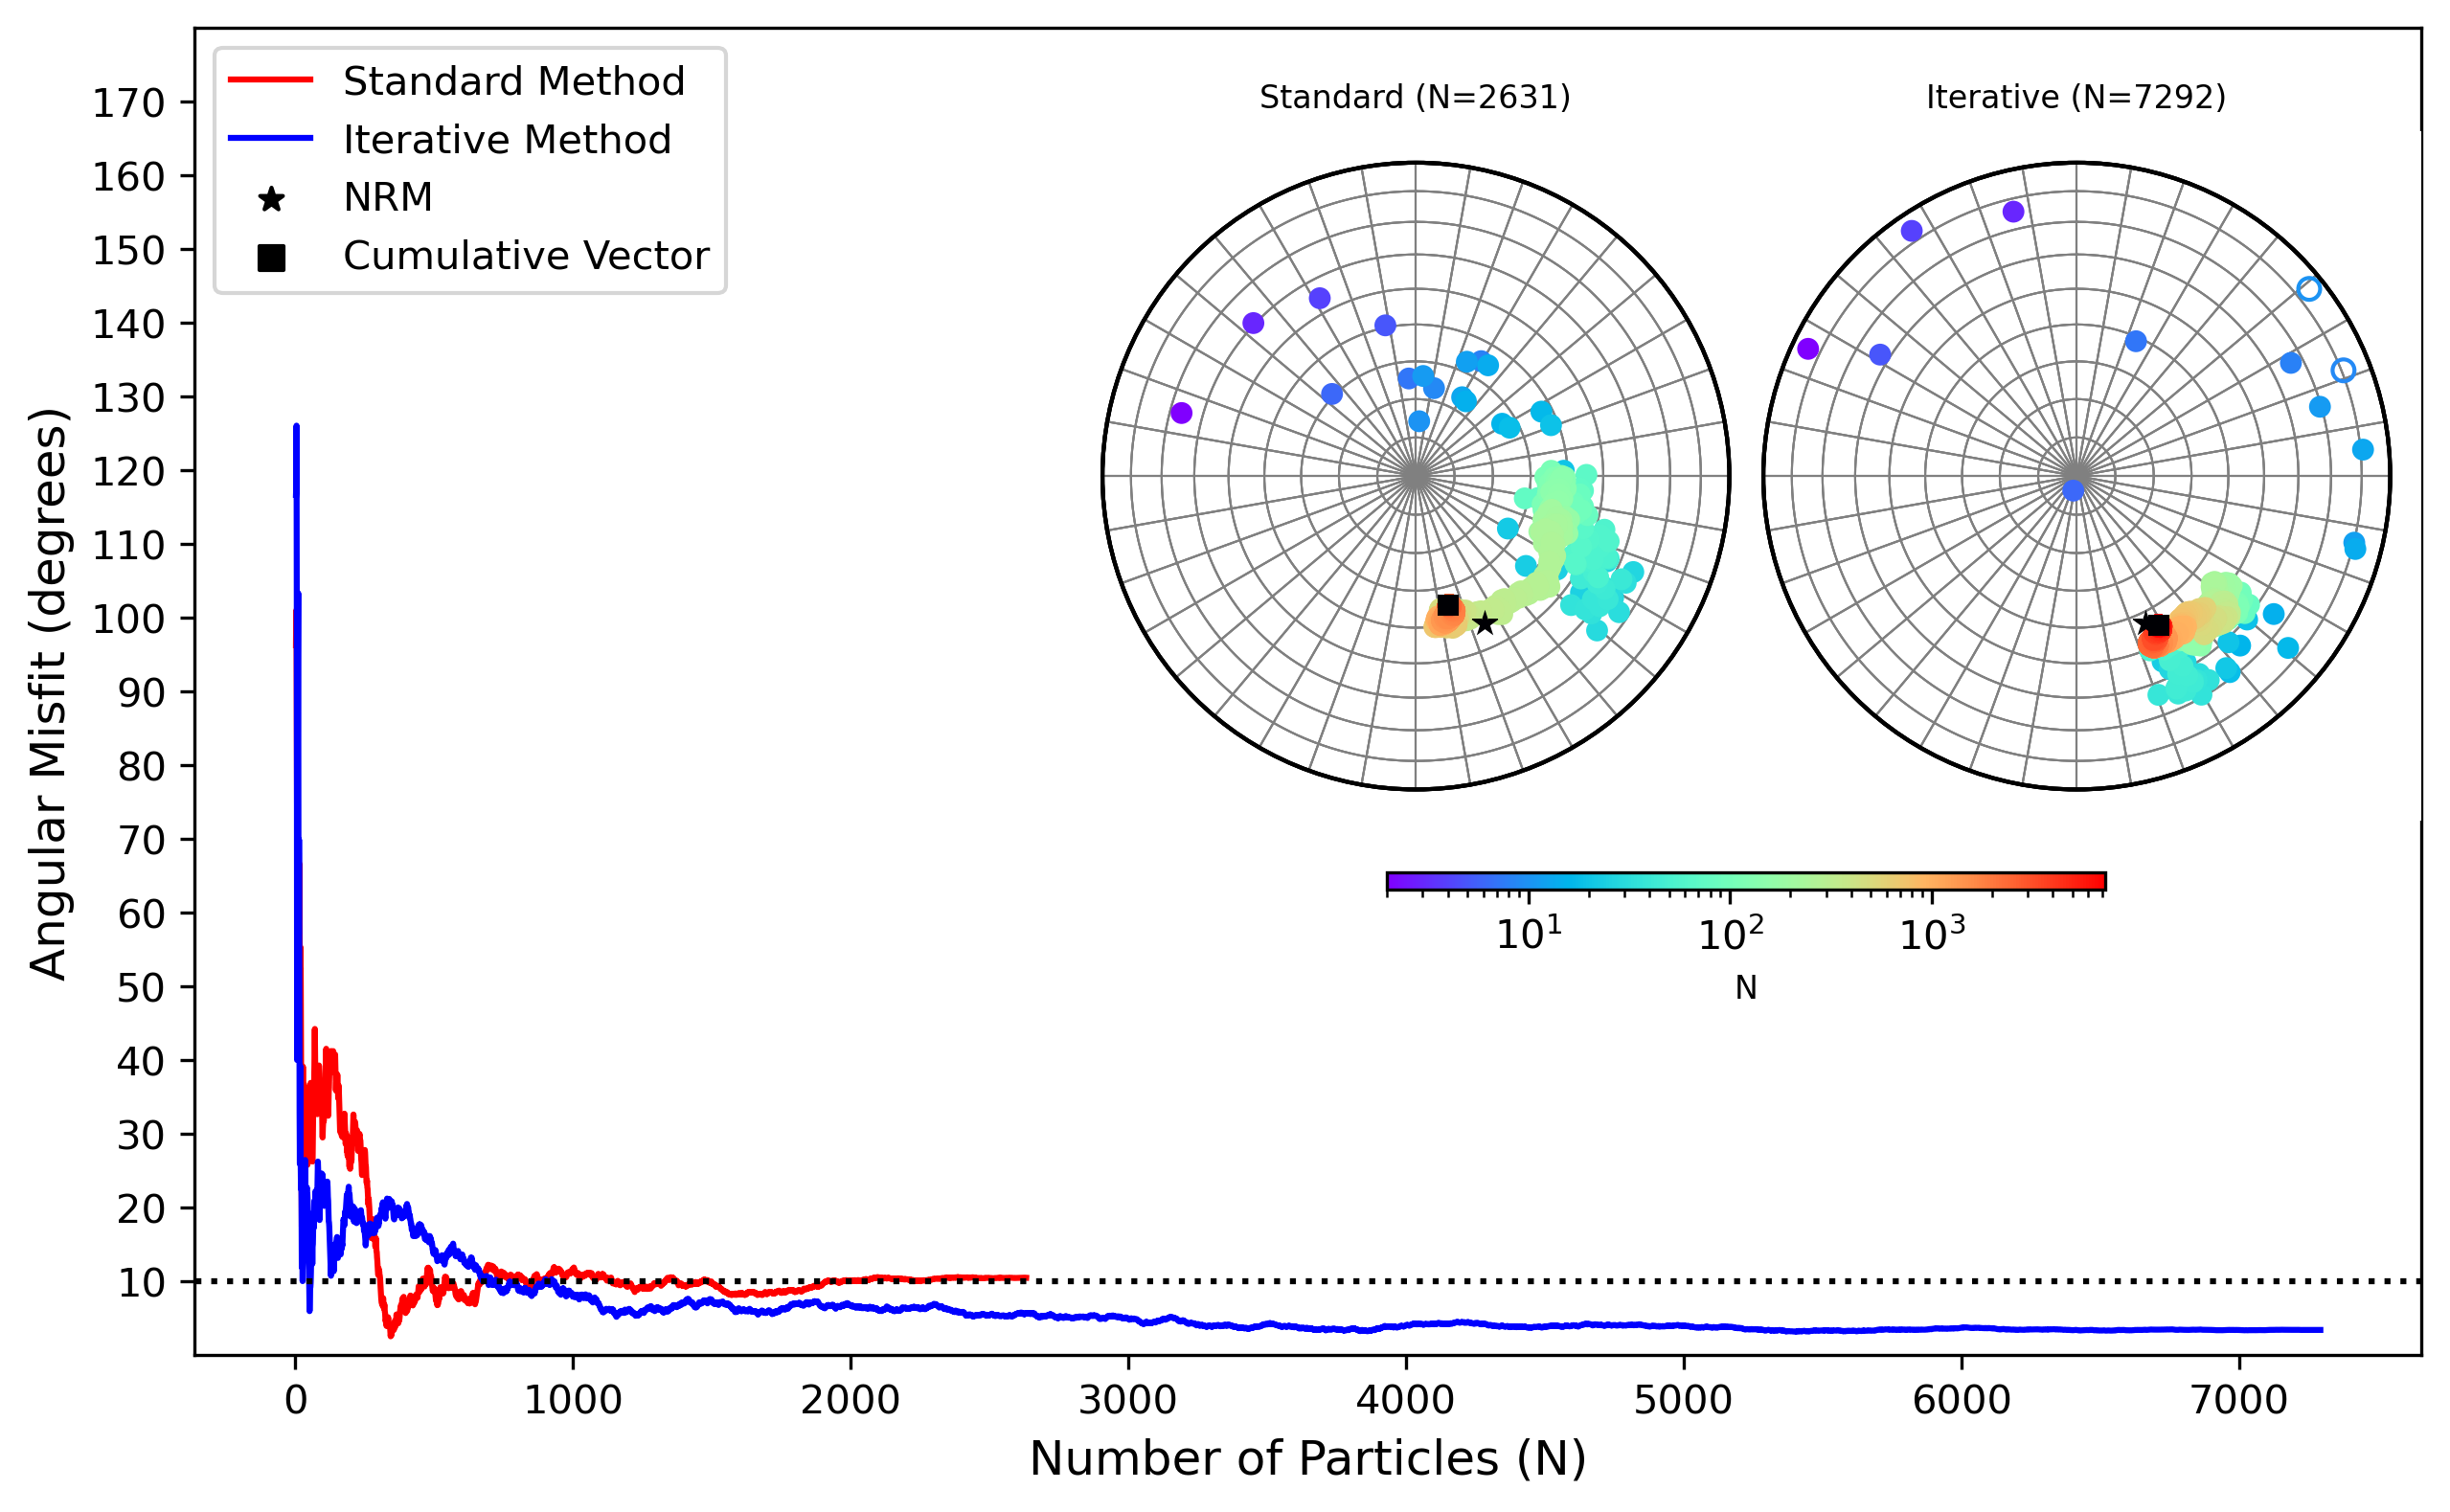
\includegraphics[width=1\linewidth]{figures/basalt-data-stereoplot.png}
  \caption{
  Comparison of the standard (red) and iterative (blue) algorithms in reconstructing the NRM direction from the basalt sample. (Left) Angular misfit between the cumulative vector and the measured NRM as a function of the number of particles ($N$). (Right) Stereographic projections of the filtered magnetic vectors ($R^2 \geq 0.9$) for both methods, with the measured NRM (star), non-filtered cumulative direction (triangle), and the filtered cumulative direction (square) indicated. The color gradient denotes the logarithmic scale of particle counts, with warmer colors representing higher concentrations. The solid-lined and dashed-lined curves represent the non-filtered and outliers filtered data, respectively.
  }
  \label{basalt-data-stereograms}
\end{figure}

%%%%%%%%%%%%%%%%%%%%%%%%%%%%%%%%%%%%%%%%%%%%%%%%%%%%%%%%%%%%%%%%%%%%%%%%%%%%%%%
\section{Discussion}

Inverting unique magnetic moment from MM data, regardless of the technique, demands knowing the position of sources. The application of the Euler deconvolution technique emerges to avoid additional measurements, such as nano-tomography, to uncover that information. The isolated windows approach, as justified by \cite{Souza-Junior2024}, enables the separation of the primary signal from the surrounding area using the total gradient anomaly. This method effectively isolates the desired signal while excluding regions outside the window boundaries, which are less sensitive to variations in the magnetic parameters of the specific source. Using this windows approach enables a rapid solution to the inversion problem while keeping it largely overdetermined, since only three parameters are solved per sliced data. However, this thresholding exclusion of the area from the inversion domain violates the basic theory of inversion, which demands that the entire system be considered, ensuring that the interactions between all sources are properly accounted for to obtain a unique and precise solution \citep{Baratchart2013, Lima2013}. Thus, the previous approach of \cite{Souza-Junior2024} will not yield reliable results in all cases. Specifically, in cases influenced by distant sources, even those that are weak, either within the window or close by, which compromises its effectiveness. The latter reflects on a higher amount of results discarded by the filtering criterion.

To tackle these challenges, the iterative method was introduced, providing a more reliable solution for mitigating interference between sources while still preserving the isolated windows approach. Naturally, this comes at the cost of increased inversion time, but the method remains efficient enough to run on a personal computer without demanding massive computational power. Despite the improvements, not all problems have been solved. The new method is more effective at detecting particles and results in more particles passing through the filtering criteria. However, it still faces challenges with inherent limitations of the Euler deconvolution, such as clustered signals. This introduces position estimation errors that are directly influenced by the particle's magnetic signal strength. In particular, errors in vertical position estimation lead to a compensatory trade-off between this positional uncertainty and the recovered dipole intensity. For this reason, our focus here is on the directional aspects of the dataset, while the intensity aspect will require more complex future experiments, along with the implementation of a more refined approach to solving Euler's homogeneity equation, as proposed by \citet{Uieda2025}.

\subsection{Directional recovery assessment}

As noted by \citet{Oliveira2015Estimation}, the least-squares estimator is less sensitive to small errors in particle position and violation of the dipolar assumption when recovering directional information (declination and inclination). This makes the new method particularly effective in refining estimates, increasing the number of results that meet the filtering criteria. As a result, the approach becomes more statistically robust, ultimately improving the overall data quality. The fitting performance was assessed using both synthetic and real datasets, requiring a reliable reference for comparison. In the case of synthetic data, a directional bias (synthetic NRM) was introduced to the dipole magnetic moments based on a spherical distribution. For real samples, the reference direction was obtained from NRM measurements of the whole thin section using the 2G magnetometer.

From the synthetic tests (Figure~\ref{synthetic-data-stereograms}a-c), both the original \citep{Souza-Junior2024} and iterative methods performed well in recovering the directional bias mainly for two reasons. First, dipolar models are generally simpler and tend to produce more results that pass the filtering criteria. Even though the standard method is less efficient in estimating parameters, this deficiency is compensated by the overall behavior of the synthetic sample, and any poor-fitting is treated as random inputs that are effectively removed in the vector sum. The second reason is that, despite a wide distribution of particle moments (from \(10^{-15}\) to \(10^{-11}\)), the stronger particles, which could have further complicated the signal, also followed the bias direction. This contrasts with the overlapping signals synthetic case (Section~\ref{sec:synthetic-overlapping}), where the strong particles were randomly oriented. Nonetheless, it serves as a proxy to isothermal remanent magnetization study cases.

For the real samples, the results in one case deviated from initial expectations. The most dispersed assembly, characterized by a higher proportion of SD/PSD grains and a lower packing density of magnetic particles, exhibited the highest angular misfit, though it remained below 10 degrees (Figure~\ref{ceramic-data-stereograms}). In contrast, the basalt sample produced an angular misfit of less than 5 degrees (Figure~\ref{basalt-data-stereograms}), a result that was not anticipated given the high particle density, particularly the presence of MD grains. This density violates a key assumption of the method, namely that each window should ideally contain a single particle \citep{Souza-Junior2024}. A possible explanation for this positively surprising behavior is provided by recent nanotomography studies of basaltic rocks \citep[\textit{e.g.}][]{Out2024, Out2025}, which have revealed clusters of magnetic particles smaller than \(1~\mu m\). When a window captures such a cluster, the recorded signal represents the sum of the individual contributions. If the cluster exhibits a directional bias, this bias is likely to be reflected in the inversion result. This effect may also account for the improved performance of the standard method in the basaltic sample. While this approach does not effectively resolve interfering sources, it can still capture the overall directional bias of clustered particles, resulting in a lower angular misfit despite the sample’s high particle density.


%%%%%%%%%%%%%%%%%%%%%%%%%%%%%%%%%%%%%%%%%%%%%%%%%%%%%%%%%%%%%%%%%%%%%%%%%%%%%%%
\section{Conclusion}

Our improved algorithm demonstrates substantial advancements over its predecessor, particularly in the context of magnetic microscopy mapping for paleomagnetic studies. By refining the isolation of the primary signal and incorporating an interfering source algorithm, we have enhanced the accuracy of 3D positioning and dipole moment estimations, addressing key limitations of the previous version. These improvements have led to better particle distribution and an increased number of particles meeting the filtering criteria, while also identifying more grains through re-detection. Consequently, the cumulative vector analysis now includes more grains, ensuring statistically reliable direction estimates. This can be achieved with particle counts ranging from several hundred to a few thousand, as demonstrated by both numerical simulations and real data. However, similar conclusions cannot be drawn for intensity studies, as limitations persist in the recovered moment for grains, particularly in clustered particles. Therefore, further research is needed to assess whether this enhanced technique can be applied to paleointensity studies. Despite these challenges, the present work represents a significant advancement in paleomagnetic research at the microscale, owing to the algorithm's ability to recover bulk directional information.

This provides an important step towards paleomagnetism using magnetic microscopy. The possibility of retrieving reliable magnetization directions from thin sections broadens the horizons of previous bulk-derived measurements, such as paleomagnetic tests (e.g., ``conglomerate'' and microscale fold tests). Not only this, we have more capability to spatially correlate the directions estimated (e.g. single crystal inclusion) by obtaining the magnetic information associated with optical images.


\section{Open research}

The Python source code used to produce all results and figures presented here,
as well as supplementary figures and Jupyter notebooks, and the QDM magnetic
microscopy data used in this study are available from \citet{figshare}, which
can also be found on \url{https://github.com/\GitHubRepository} under the MIT
(source code) and CC-BY (data, text, and figures) licenses.

We made use of the following Python software in our research:
scikit-image \citep{VanderWalt2014} for image processing and blob detection;
matplotlib \citep{Hunter2007} for generating figures and stereograms;
Numpy \citep{Harris2020} for basic linear-algebra and array computations;
Scipy \citep{2020SciPy-NMeth} for linear-algebra and non-linear optimization;
Verde \citep{verde2018} for generating data grids;
Harmonica \citep{harmonica2020} for upward continuation and magnetic data processing;
Choclo \citep{choclo2022} for optimized kernel functions used in the
forward and inverse modeling;
Numba \citep{lam2015numba} for just-in-time compilation;
xarray \citep{hoyer2017xarray} for coordinate-aware multidimensional arrays.

%%%%%%%%%%%%%%%%%%%%%%%%%%%%%%%%%%%%%%%%%%%%%%%%%%%%%%%%%%%%%%%%%%%%%%%%%%%%%%%
\section{Acknowledgements}

We gratefully acknowledge the Laboratório de Paleomagnetismo e Magnetismo de Rochas (USPmag, Universidade de São Paulo) for maintaining and providing access to samples, and the Harvard Paleomagnetics Lab (Department of Earth and Planetary Sciences, Harvard University) for providing the facilities and equipment used for the QDM and bulk measurements. We sincerely acknowledge the developers and maintainers of the open-source software, whose contributions were essential to the completion of this work. This research was supported by grants 2021/08379-5 and 2023/13372-5 from the Fundação de Amparo à Pesquisa do Estado de São Paulo (FAPESP), grant IES\textbackslash{}R3\textbackslash{}213141 from the Royal Society, and grant PRPI 22.1.09345.01.2 from Universidade de São Paulo.
The opinions, hypotheses, and conclusions or recommendations expressed in this material are the responsibility of the authors and do not necessarily reflect the views of FAPESP.




\bibliographystyle{apalike-doi}
\bibliography{references}

\end{document}
